\documentclass[12pt]{article}\usepackage[]{graphicx}\usepackage[]{color}
%% maxwidth is the original width if it is less than linewidth
%% otherwise use linewidth (to make sure the graphics do not exceed the margin)
\makeatletter
\def\maxwidth{ %
  \ifdim\Gin@nat@width>\linewidth
    \linewidth
  \else
    \Gin@nat@width
  \fi
}
\makeatother

\definecolor{fgcolor}{rgb}{0.345, 0.345, 0.345}
\newcommand{\hlnum}[1]{\textcolor[rgb]{0.686,0.059,0.569}{#1}}%
\newcommand{\hlstr}[1]{\textcolor[rgb]{0.192,0.494,0.8}{#1}}%
\newcommand{\hlcom}[1]{\textcolor[rgb]{0.678,0.584,0.686}{\textit{#1}}}%
\newcommand{\hlopt}[1]{\textcolor[rgb]{0,0,0}{#1}}%
\newcommand{\hlstd}[1]{\textcolor[rgb]{0.345,0.345,0.345}{#1}}%
\newcommand{\hlkwa}[1]{\textcolor[rgb]{0.161,0.373,0.58}{\textbf{#1}}}%
\newcommand{\hlkwb}[1]{\textcolor[rgb]{0.69,0.353,0.396}{#1}}%
\newcommand{\hlkwc}[1]{\textcolor[rgb]{0.333,0.667,0.333}{#1}}%
\newcommand{\hlkwd}[1]{\textcolor[rgb]{0.737,0.353,0.396}{\textbf{#1}}}%

\usepackage{framed}
\makeatletter
\newenvironment{kframe}{%
 \def\at@end@of@kframe{}%
 \ifinner\ifhmode%
  \def\at@end@of@kframe{\end{minipage}}%
  \begin{minipage}{\columnwidth}%
 \fi\fi%
 \def\FrameCommand##1{\hskip\@totalleftmargin \hskip-\fboxsep
 \colorbox{shadecolor}{##1}\hskip-\fboxsep
     % There is no \\@totalrightmargin, so:
     \hskip-\linewidth \hskip-\@totalleftmargin \hskip\columnwidth}%
 \MakeFramed {\advance\hsize-\width
   \@totalleftmargin\z@ \linewidth\hsize
   \@setminipage}}%
 {\par\unskip\endMakeFramed%
 \at@end@of@kframe}
\makeatother

\definecolor{shadecolor}{rgb}{.97, .97, .97}
\definecolor{messagecolor}{rgb}{0, 0, 0}
\definecolor{warningcolor}{rgb}{1, 0, 1}
\definecolor{errorcolor}{rgb}{1, 0, 0}
\newenvironment{knitrout}{}{} % an empty environment to be redefined in TeX

\usepackage{alltt}

\usepackage{amssymb,amsmath}
\usepackage{enumerate}
\usepackage{float}
\usepackage{verbatim}
\usepackage{setspace}
\usepackage{multicol}

%% LaTeX margin settings:
  \setlength{\textwidth}{7.0in}
\setlength{\textheight}{9in}
\setlength{\oddsidemargin}{-.5in}
\setlength{\evensidemargin}{0in}
\setlength{\topmargin}{-1.5cm}

%% tell knitr to use smaller font for code chunks
\def\fs{\footnotesize}
\def\R{{\sf R}}
\newcommand{\bfbeta}{\mbox{\boldmath $\beta$}}
\newcommand{\bfD}{\mbox{\boldmath $D$}}
\newcommand{\bfL}{\mbox{\boldmath $L$}}
\newcommand{\bfR}{\mbox{\boldmath $R$}}
\newcommand{\bfmu}{\mbox{\boldmath $\mu$}}
\newcommand{\bfv}{\mbox{\boldmath $V$}}
\newcommand{\bfX}{\mbox{\boldmath $X$}}
\newcommand{\bfy}{\mbox{\boldmath $y$}}
\newcommand{\bfb}{\mbox{\boldmath $b$}}
\IfFileExists{upquote.sty}{\usepackage{upquote}}{}
\begin{document}


  
  
\begin{center}
\large{Bayes: Homework $2$} \\
Leslie Gains-Germain
\end{center}

\begin{doublespacing}

\begin{enumerate}

\item The mathematical definition of probability out of Casella and Berger's {\it Statistical Inference}:

{\it Given a sample space S and an associated sigma algebra B, a probability function is a function P with domain B that satisfies
\begin{enumerate}
\item $P(A) \geq 0$ for all $A \in B$
\item $P(S) = 1$ 
\item $If A_1, A_2,...\in B$ are pairwise disjoint, then $P(\cup_{i=1}^{\infty}A_i) = \sum_{i=1}^{\infty}P(A_i)$
\end{enumerate}}

Two ways that we use probability to summarize the world around us: 
\begin{itemize}
\item We use probabilities to describe how likely an outcome is in a game of chance. For example, if we roll a fair die and we have no knowledge of the outcome, the probability of rolling a $3$ is $1/6$. We can also assign probabilities to the outcomes of flipping a coin, spinning a spinner, or picking a random card from a deck.
\item The second way we use probabilities is to describe our degree of certainty about something happening in the future. For example, I might say to my boyfriend, ``There is a $10\%$ chance that I will do the dishes tonight.'' I am trying to convey to him that it is not very likely that I will be doing the dishes, and I use the words ``probability'' and ``chance'' to convey that idea. I don't necessarily want to completely rule out the possibility of me doing the dishes, because I figure there is a 'chance' that he will become injured during the day. Even when I'm trying to remember something, like the name of someone from my childhood, I'll catch myself saying something like, ``I'm $99\%$ sure that her name was Nina.'' Sometimes, our use of probability can be based on something more concrete but is still used to convey uncertainty. For example, suppose I say that the chance Serena Williams will win the US open is $90\%$. I'm basing this off her previous performance this calendar year, and I'm using that as reasoning for my degree of certainty in the outcome of the tournament.
\end{itemize}

\item A frequentist's criticism of the likelihood principle is that likelihood inference about model parameters is the same in two studies with different designs but the same sample data. Consider the example given on the Wikipedia page for the Likelihood principle. Let X be a random variable that represents that number of heads in 12 flips of an unfair coin, where $\theta$ is the probability of heads in each trial. Then $X \sim Bin(12, \theta)$. If the experiment is conducted and we observe 3 heads, $X=3$, then the likelihood function is as follows:

\begin{align*}
L(\theta|X=3) &= {12 \choose 3}\theta^3(1-\theta)^9=220 \theta^3 (1-\theta)^9
\end{align*}

Now, let Y be the number of flips needed to get three heads. If we observe the same sample data as the previous example, then $Y=12$. The likelihood function for this example is as follows:

\begin{align*}
L(\theta|Y=12) &= {11 \choose 2}\theta^3(1-\theta)^9=55 \theta^3 (1-\theta)^9
\end{align*}

The first likelihood function is a scalar multiple of the second, so inference about the probability of getting heads, $\theta$, is exactly the same in these two scenarios (the estimates will be the same and likelihood based confidence intervals will be the same). This is consistent with the likelihood principle because the observed data are the same in both cases (three success in 12 flips, or 12 flips to get three successes). Frequentists argue, however, that the study design - whether we count the number of flips needed to get three heads or the number of heads in 12 flips - should be considered when making inference about $\theta$.

\item See attached handwritten sheet.

\item I am going to use a simple example to explain this concept to someone with little mathematical background. Say you are given an unfair coin, and the probability of getting heads is $\theta$. The natural way to learn something about $\theta$ is to pick up the coin and start flipping it. The proportion of heads you get in $10$ tosses is clearly going to be your best guess for $\theta$. This is exactly what the likelihood function does, it tells us how likely values of $\theta$ are given observed sample data. The likelihood function, $L(\theta|x)$, is a function of $\theta$ and gives us a likelihood for each possible value of $\theta$, given that the sample data have been observed and are fixed. In the example, suppose we observe $8$ heads in $10$ tosses of the coin. Then the likelihood function will tell us that the most likely value for $\theta$ is $8/10$ or $4/5$. Values such as $7/10$ and $9/10$ will be likely (although slightly less likely than $4/5$), and and a value such as $1/10$ will not be likely at all. A probability distribution, on the other hand, describes the probability of observing sample data, given the value of $\theta$ is fixed. In the example given, suppose we knew that the probability of getting heads with the unfair coin was $3/4$. Then we could calculate the probability of getting $1, 2, 3, 4, ....,$ or $10$ heads in $10$ tosses of the coin, given that the probability is $3/4$ on each flip. The difference between the likelihood function and the probability function lies in what we think about as fixed and what we think about as varying. The sample data varies in a probability function with $\theta$ fixed, and $\theta$ varies in a likelihood function, with the sample data fixed.

\item Suppose that the true probability of duckling survival is $\theta=1/2$. Then the probability that all $24$ ducklings survive in a week is $1/24^2$, a number very close to zero. Frequentists would estimate $\theta$ to be $1$, the observed proportion of birds that survived. This estimate doesn't make sense because everyone knows bird survival rate is not $1$. Likelihoodists would also estimate $\theta$ to be $1$ - the MLE. In both frequentist and likelihoodist land, the estimates for $\theta$ are nonsense because of this one bad sample. In Bayesian land, the unrepresentative sample will still influence estimates, but at least the sample is not the {\it only} piece of information going into the posterior predictive distribution. For example, if we use a Beta(2,2) prior, the posterior distribution, would be a Beta(26,2). The estimator for $\theta$ under squared error loss is then $26/28=0.93$. This estimator is still off, but at least it makes more sense than the likelihood and frequentist estimator of $1$. Note: it turns out that if we were to construct uncertainty intervals, none of the three methods would capture the true value of $\theta$, but the Bayesian interval would probably be closer to capturing the truth.



\item A plot of beta distributions with four different parameter values of $\alpha=\beta$ is shown below.

\begin{center}
\begin{knitrout}\footnotesize
\definecolor{shadecolor}{rgb}{0.969, 0.969, 0.969}\color{fgcolor}
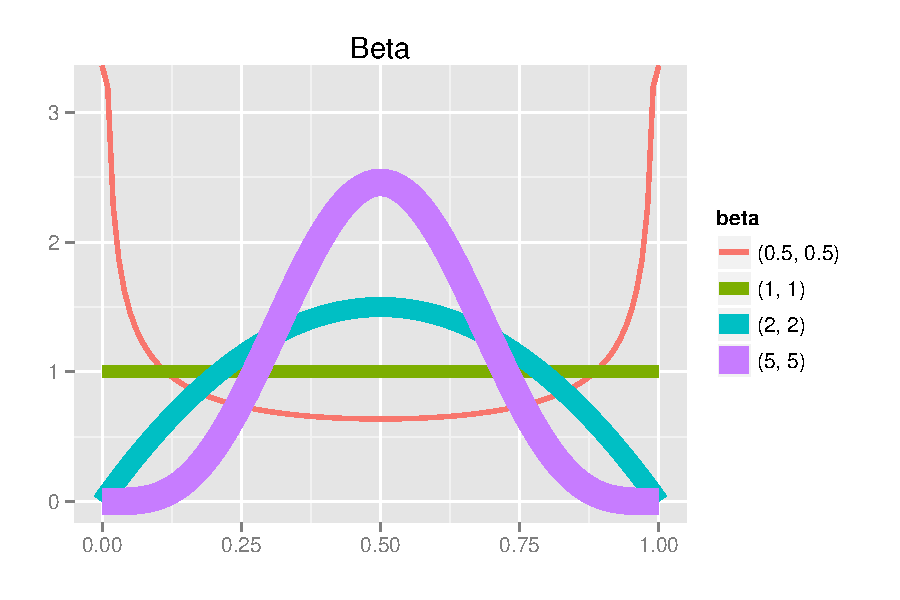
\includegraphics[width=0.8\linewidth]{figure/betaplot-1} 

\end{knitrout}
\end{center}

\item Note that the parameterization of the gamma distribution given by Gelman et. al is technically a gamma* distribution on Boik's equation sheet. This means that when Gelman talks about a Gam(1/2, 1/2), he is really talking about a Gam*(1/2, 1/2) which is a Gam(2, 2) distribution according to Boik, R, Wikipedia, and most everyone else. In the plot below, I am using Gelman's parameterization. A gamma prior is often used for the precision parameter (1/variance) in a normal distribution. For example, if we want large values of the variance most likely, then we choose a Gam(2, 2) prior for the precision. This makes small values of the precision and large values of the variance most likely. The distribution of the variance (1/precision) follows an inverse gamma distribution, which also has nice properties. I think the gamma distribution is a natural choice as a prior for the precision because of the shape of the distribution. If we choose a Gam(1,1) or a Gam(2,2) prior on the precision, small values of the precision are the most likely, and larger values of the precision are less and less likely. By changing the parameters of the gamma distribution, we can change how much weight we want to put on small and large values of the precision. \\

I'm guessing that Gelman uses a different parameterization for the gamma distribution than most to help the user remember what prior to choose if he/she wants to make large values of the variance most likely. The larger the $\alpha, \beta$ parameters in Gelman's parameterization of the gamma prior makes {\it larger} values of the variance more likely. With Boik's parameterization of the Gamma distribution, you would need to use a gamma prior with {\it smaller} parameter values to make larger values of the variance more likely.


\begin{center}
\begin{knitrout}\footnotesize
\definecolor{shadecolor}{rgb}{0.969, 0.969, 0.969}\color{fgcolor}
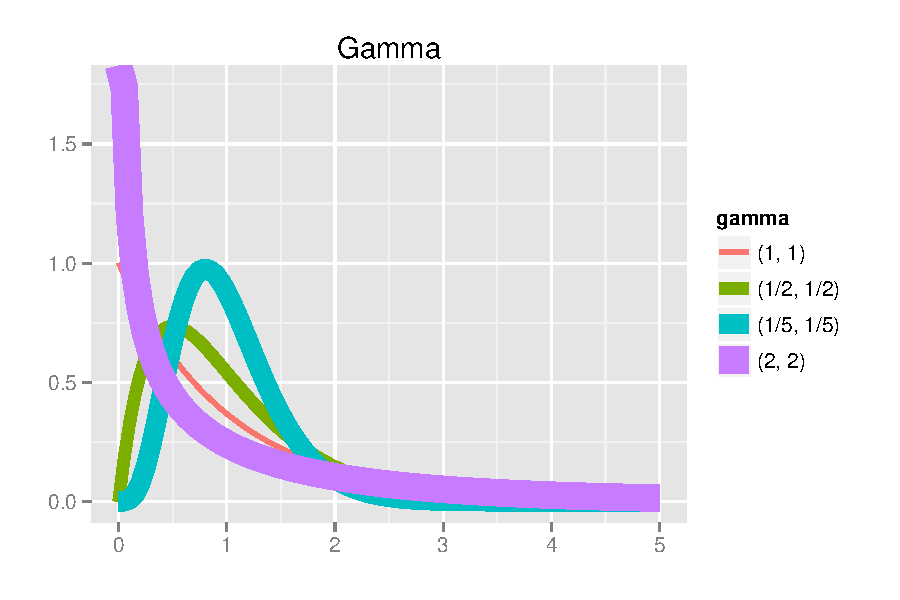
\includegraphics[width=0.8\linewidth]{figure/gammaplot-1} 

\end{knitrout}
\end{center}

\item \begin{enumerate}

\item See my work below. The probability of being infected if the person tests positive is $0.326$ for Doctor $1$'s belief and $0.505$ for Doctor $2$'s belief about the infection rate.

\begin{align*}
P(disease|test pos) &= \frac{P(test pos and diseased)}{P(test pos)} \\
&= \frac{P(test pos|disease)P(disease)}{P(test pos|disease)P(disease)+P(test pos|no disease)P(no disease)} \\
Doc 1 &= \frac{0.92*.05}{0.92*0.05+0.10*0.95} = 0.326 \\
Doc 2 &= \frac{0.92*.10}{0.92*0.10+0.10*0.90} = 0.505
\end{align*}

\item I chose to use a normal prior distribution to reflect each Doctor's belief. I chose the mean to be $0.05$ and $0.10$ for each doctor, respectively. I chose the standard deviation so that their beliefs would not overlap too much. It looks like Doctor $1$ would think of $3-7\%$ as reasonable values, and Doctor $2$ would think of $8-12\%$ as reasonable values for the infection rates.  

\begin{center}
\begin{knitrout}\footnotesize
\definecolor{shadecolor}{rgb}{0.969, 0.969, 0.969}\color{fgcolor}
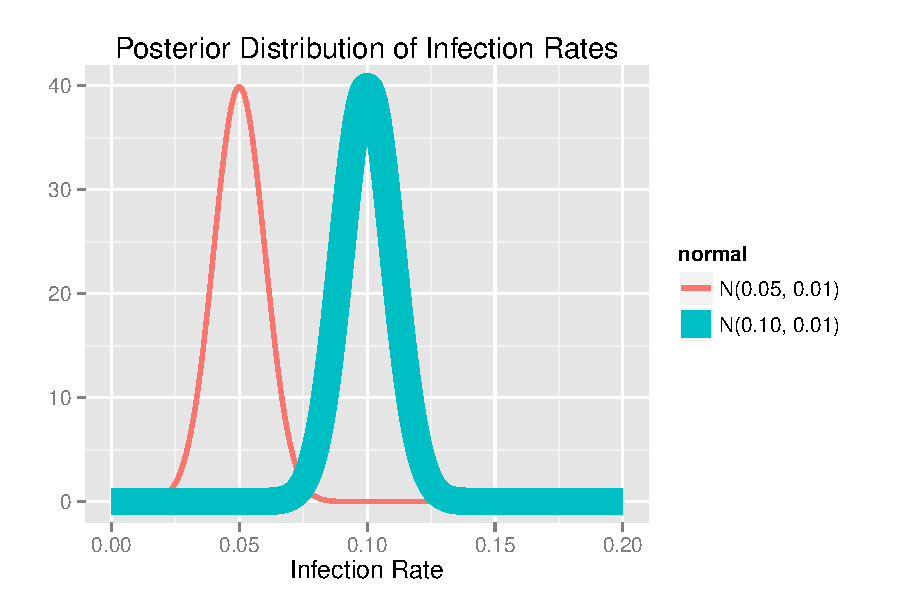
\includegraphics[width=0.8\linewidth]{figure/normplot-1} 

\end{knitrout}
\end{center}
\end{enumerate}

\item Based off what I could find about this first Bayesian analysis done by Laplace, it sounds like he used a weakly informative Beta(2,2) prior for $\theta$. Below, I use Bayes rule to find the posterior distribution of $\theta$ based on the birth data from Laplace's time. Let X be the number of female births out of the $493472$ births in Paris from $1745$ to $1770$. Let $\theta$ represent the probability that any birth is female. Then, by Bayes rule:

\begin{align}
P(\theta|X=x) &= \frac{p(x|\theta)p(\theta)}{p(x)} \\
&= \frac{{493472 \choose x}\theta^x(1-\theta)^{493472-x}*6\theta(1-\theta)}{\int_{0}^{1}{493472 \choose x}\theta^x(1-\theta)^{493472-x}*6\theta(1-\theta)d\theta} \\
&= \frac{6{493472 \choose x}\theta^{x+1}(1-\theta)^{493473-x}}{6{493472 \choose x}*\beta(x+2, 493474-x)\int_{0}^{1}\frac{\theta^{x+1}(1-\theta)^{493473-x}}{\beta(x+2, 493474-x)}} \label{int} \\ 
&= \frac{\theta^{x+1}(1-\theta)^{493473-x}}{\beta(x+2, 493474-x)}
\end{align}

Note that the integral is equal to $1$ in line \ref{int}, because we integrate the pdf for a Beta(x+2, 493474-x) distribution. We then find that the posterior distribution for $\theta$, given the observed $X=241945$, is a $Beta(241947, 251529)$ distribution. This distribution is plotted below, the mean is $241947/493476=0.4902913$, and the standard deviation is approximately $0.0007$. The mean is only very slightly larger than the observed proportion of girls in the sample, $241945/493472=0.4902912$. The probability that $\theta$ is less than $0.5$ is very very close to $1$ because almost all of the density of the posterior probability distribution for $\theta$ lies below $0.5$. There is very strong evidence that $\theta$ is  less than $0.5$. 


\begin{knitrout}\footnotesize
\definecolor{shadecolor}{rgb}{0.969, 0.969, 0.969}\color{fgcolor}
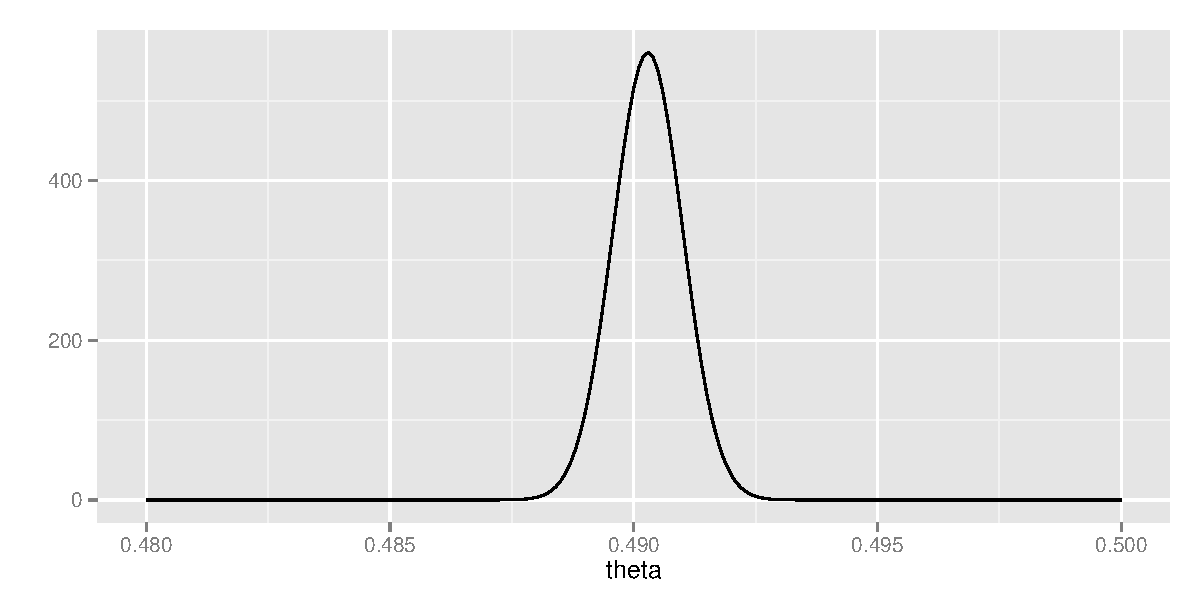
\includegraphics[width=0.8\linewidth]{figure/singlebetaplot-1} 

\end{knitrout}

\item  \begin{enumerate}
\item In the plot below, the dashed line is the mle, which is also the mean of the likelihood function, $4.85$. The endpoints of the $95\%$ confidence interval are $3.74$ and $6.16$. These endpoints were found by find the values of $\lambda$ that have a likelihood that is $5\%$ of the likelihood at the mle.

\begin{knitrout}\footnotesize
\definecolor{shadecolor}{rgb}{0.969, 0.969, 0.969}\color{fgcolor}
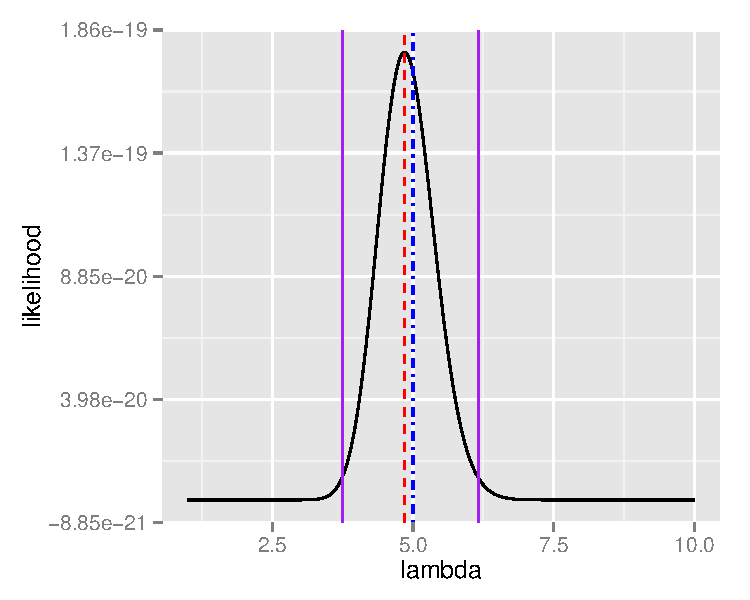
\includegraphics[width=.5\linewidth]{figure/poisson20-1} 

\end{knitrout}


\item With a sample size of $100$ observations, the mle is $4.83$, and the endpoints of the $95\%$ likelihood interval are $4.31$ and $5.39$. Although the accuracy of the mle has not improved, the width of the interval has decreased.

\begin{knitrout}\footnotesize
\definecolor{shadecolor}{rgb}{0.969, 0.969, 0.969}\color{fgcolor}
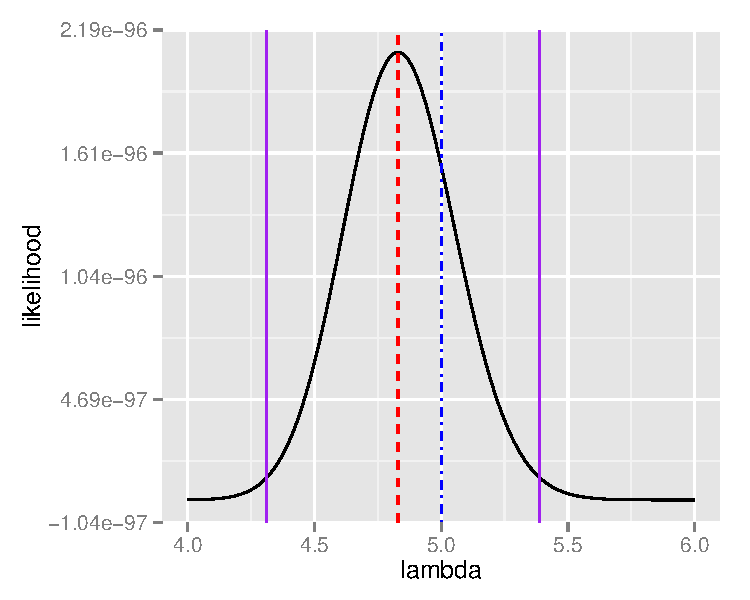
\includegraphics[width=.5\linewidth]{figure/poisson100-1} 

\end{knitrout}

\item The contour plot is shown below. The mles were found by maximizing the three dimensional likelihood surface with respect to $\mu$ and $\sigma^2$. With a sample size of $15$ observations, the mle for $\mu$ is $9.17$, and the mle for $\sigma^2$ is $3.30$. The {\it profile} $95\%$ confidence intervals are $(8.03, 10.32)$ and $(1.51, 9.42)$ for $\mu$ and $\sigma^2$ respectively.

\begin{knitrout}\footnotesize
\definecolor{shadecolor}{rgb}{0.969, 0.969, 0.969}\color{fgcolor}
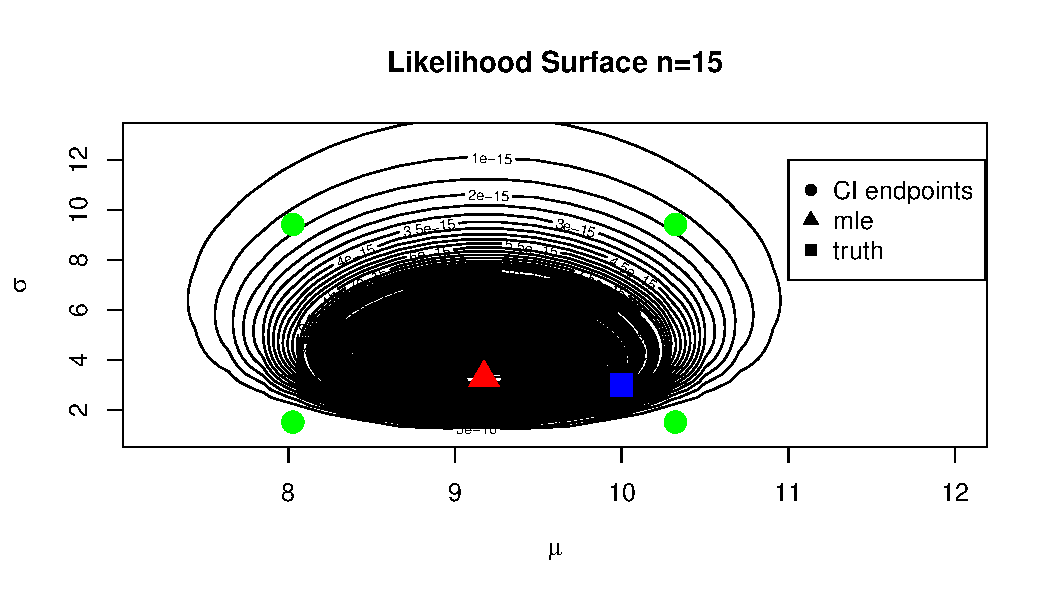
\includegraphics[width=0.8\linewidth]{figure/normal15-1} 

\end{knitrout}

\item With a sample size of $5$, the mles are farther from the truth, and neither of the profile confidence intervals contain their respective true value. The mle for $\mu$ is $8.81$ and the mle for $\sigma^2$ is $1.05$. The $95\%$ profile confidence interval for $\mu$ is $(7.69, 9.94)$, and the $95\%$ profile confidence interval for $\sigma^2$ is $(0.48, 3.01)$.

\begin{knitrout}\footnotesize
\definecolor{shadecolor}{rgb}{0.969, 0.969, 0.969}\color{fgcolor}
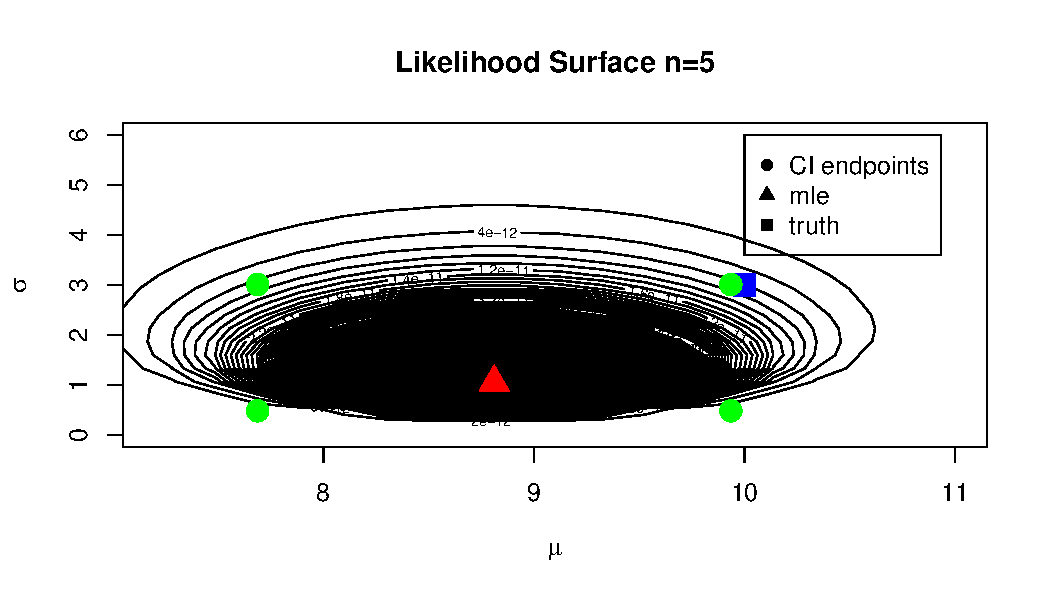
\includegraphics[width=0.8\linewidth]{figure/normal5-1} 

\end{knitrout}

\item For the binomial likelihood, I assumed that $m$ was fixed at $100$ and found the MLE for $p$. The MLE for p was $0.2$ (the same as the truth) because it just so happened that in the sample drawn, there were $20$ successes. The $95\%$ confidence interval for $p$ is $0.11$ to $0.31$. 

\begin{knitrout}\footnotesize
\definecolor{shadecolor}{rgb}{0.969, 0.969, 0.969}\color{fgcolor}
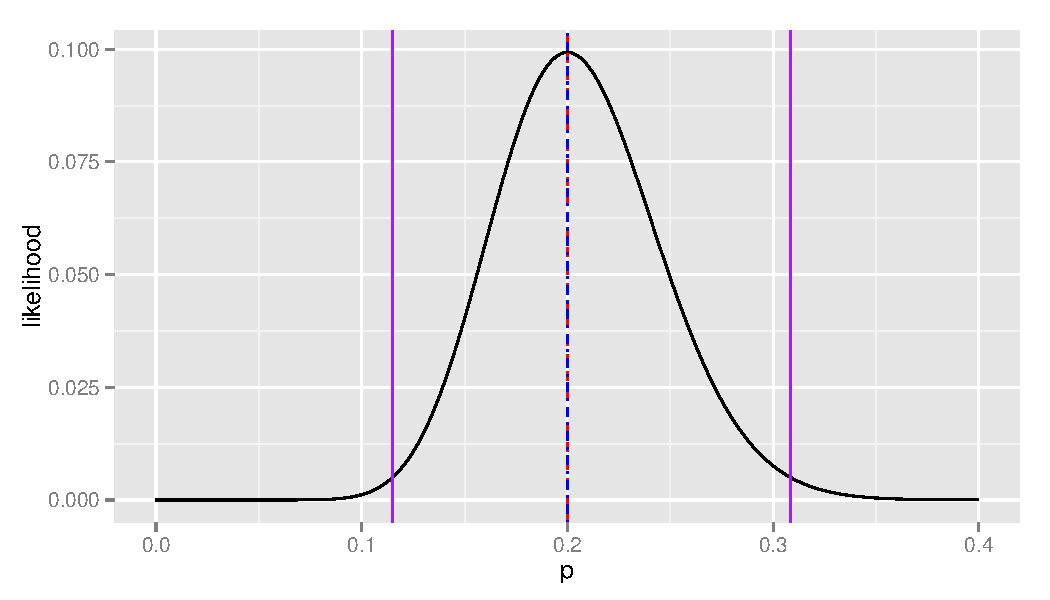
\includegraphics[width=0.8\linewidth]{figure/binom1-1} 

\end{knitrout}

\item Again, I assumed that $m$ was fixed at $100$ and found the MLE for $p$. The MLE for p was $0.19$, which is actually farther from the truth than the sample of $1$. But, the $95\%$ confidence interval for $p$ is much narrower ($0.17$, $0.21$). 

\begin{knitrout}\footnotesize
\definecolor{shadecolor}{rgb}{0.969, 0.969, 0.969}\color{fgcolor}
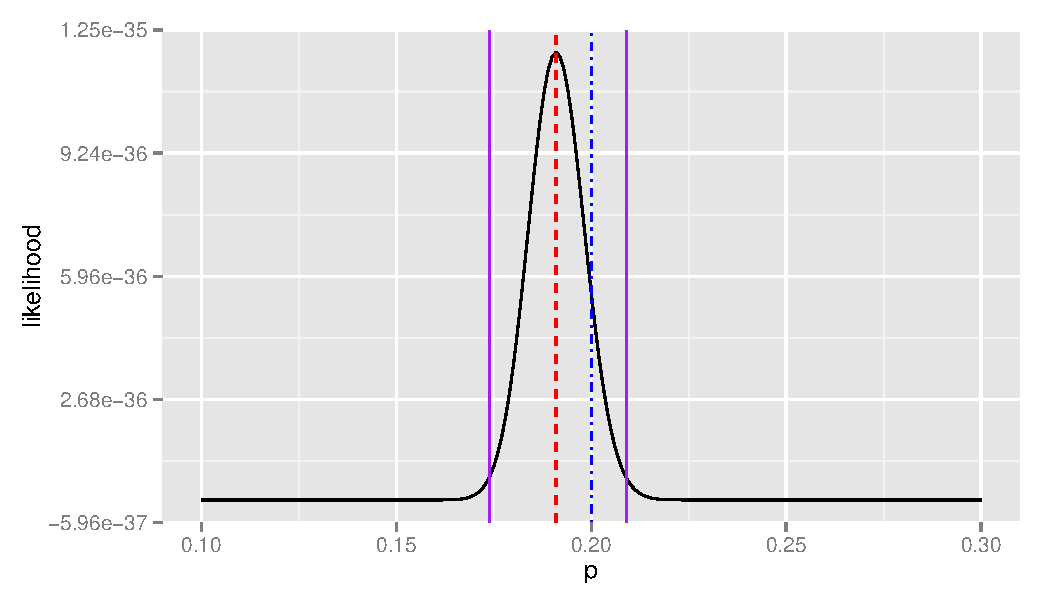
\includegraphics[width=0.8\linewidth]{figure/binom30-1} 

\end{knitrout}

\end{enumerate}

\newpage

\item \begin{enumerate}
\item The formula for the marginal probability density for $y$ is shown below, as well as the density curve.
\begin{align*}
p(y) &= \sum_{\theta \in (1,2)}p(\theta, y)=\sum_{\theta \in (1,2)}p(y|\theta)p(\theta) \\
&= \frac{1}{2\sqrt{2\pi}}e^{-(y-1)^2/8}*0.5+\frac{1}{2\sqrt{2\pi}}e^{-(y-2)^2/8}*0.5 \\
&= \frac{1}{4\sqrt{2\pi}}(e^{-(y-1)^2/8}+e^{-(y-2)^2/8})
\end{align*}

\begin{center}
\begin{knitrout}\footnotesize
\definecolor{shadecolor}{rgb}{0.969, 0.969, 0.969}\color{fgcolor}
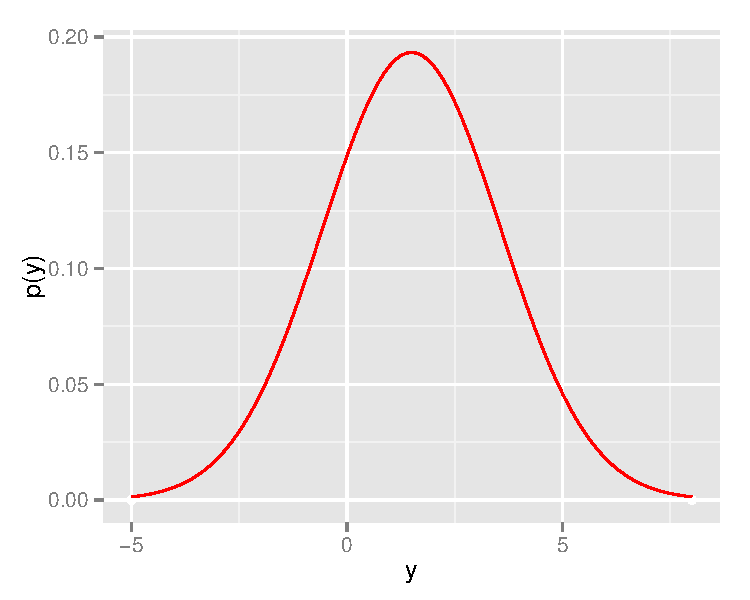
\includegraphics[width=.5\linewidth]{figure/marginalplot-1} 

\end{knitrout}
\end{center}

\item See work below.
\begin{align*}
P(\theta=1|Y=1) &= \frac{P(Y=1|\theta=1)P(\theta=1)}{P(Y=1)} \\
&= \frac{\frac{1}{2\sqrt{2\pi}}*0.5}{{\frac{1}{4\sqrt{2\pi}}(1+e^{-1/8})}}\\
&= \frac{1}{1+e^{-1/8}} = 0.54
\end{align*}

Note that the posterior distribution of theta is a probability distribution with all its mass at $\theta=1$ and $\theta=2$. When $\sigma=2$, the distribution of $\theta$ given $y=1$ looks like:

\begin{center}
\begin{knitrout}\footnotesize
\definecolor{shadecolor}{rgb}{0.969, 0.969, 0.969}\color{fgcolor}
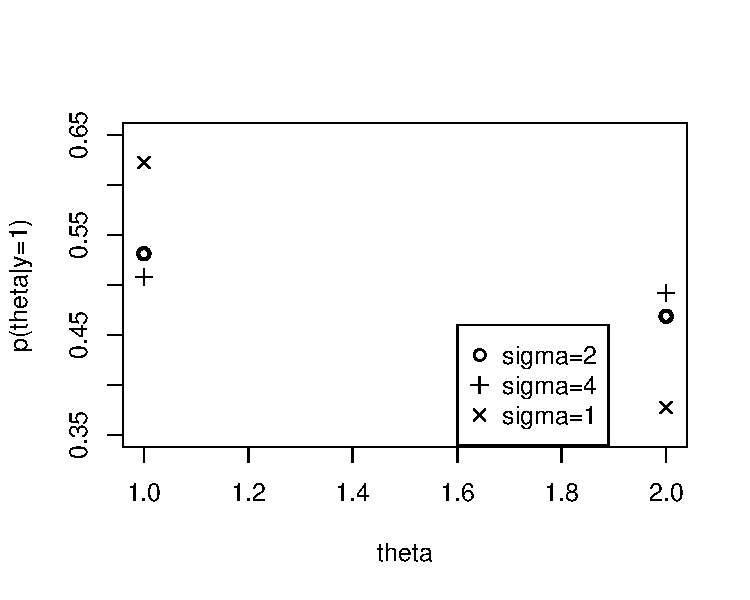
\includegraphics[width=0.5\linewidth]{figure/plotdist-1} 

\end{knitrout}
\end{center}

If we increase $\sigma$ to $4$, then $P(\theta=1|Y=1) = \frac{1}{(1+e^{-1/32})}=0.51$ and $P(\theta=2|Y=1) = \frac{e^{-1/32}}{(1+e^{-1/32})}=0.49$. If we decrease $\sigma$ to $1$, then  $P(\theta=1|Y=1) = \frac{1}{(1+e^{-1/2})}=0.62$ and $P(\theta=2|Y=1) = \frac{e^{-1/2}}{(1+e^{-1/2})}=0.38$. This is shown on the above plot. What we see is that as $\sigma$ decreases, the posterior density becomes more concentrated at $\theta=1|Y=1$ and less concentrated at $\theta=2|Y=1$. This means that the posterior probability of $\theta=1$ is larger for smaller $\sigma$. The opposite is true as $\sigma$ increases. For larger $\sigma$, the posterior probability is greater for $\theta=2|Y=1$ and less for $\theta=1|Y=1$. It looks like the $P(\theta=1|Y=1)$ and $P(\theta=2|Y=1)$ is approaching $0.5$ as $\sigma$ increases. 

\end{enumerate}

\item The probability that Elvis is an identical twin, given that he has a twin brother, is $\frac{5}{11}$.
\begin{align*}
P(identical twins|twin brother) &= \frac{P(identical twins, twin brother)}
{P(twin brother)} \\
&= \frac{P(twin brother| identical twins)P(identical twins)}{P(twin brother)}\\
&= \frac{\frac{1}{2}\frac{1}{300}}{\frac{1}{2}\frac{1}{300}+\frac{1}{4}\frac{1}{225}}
= \frac{5}{11}
\end{align*}

\item \begin{enumerate}

\item Let E=event that a $6$ is rolled. Let $I_A$=knowledge of the outcome of the roll and $I_E$=no knowledge. Then $P(E|I_E)$ would be $1/6$ because person E has no knowledge, so her best guess is to assume equal probability for all the possible outcomes of the roll. $P(E|I_A)$, however, would be either a $0$ or a $1$ depending on whether a $6$ was rolled or not. So, by the definition of subjective probability given here, the probability of rolling a $6$ would be considered subjective. Persons A and B are both rational, and they have assigned unequal probabilities to event E, conditional upon the knowledge they each have of the event. 

\item Let event E be the event that Brazil wins the next World Cup. If A is ignorant of soccer knowledge, she would probably give all the teams equal probability of winning the World Cup, so that $P(E|I_A)=\frac{1}{no.teams playing World Cup}$. If B is knowledgeable about soccer, B knows that Brazil usually has a very good soccer team and has won the World Cup {\it five} times. Person B might weight each teams probability of winning the World Cup by their number of previous wins. In this case, person B would give Brazil a much higher probability of winning than a country less well known for soccer such as South Africa. Again, persons A and person B are both rational, and they are both assigning reasonable probabilities to even E based on their current knowledge. By the definition of subjective given here, the probability of Brazil winning the World Cup would be considered subjective. 

\end{enumerate}

\item \begin{enumerate} \setcounter{enumii}{1} 
\item We showed in class that if we have a binomial pmf and a Beta(1,1) prior, then the posterior distribution is a Beta(y+1, n-y+1). In problem $9$, I showed the steps I would go through to prove that the posterior distribution for $\theta$ wth $\alpha$ and $\beta$ unknown is $Beta(y+\alpha, n-y+\beta)$. This means that our posterior mean of $\theta$ is $\frac{y+\alpha}{n+\alpha+\beta}$. Now we must show that this posterior mean will always be between the prior mean, $\frac{\alpha}{\alpha+\beta}$ and the observed proportion of heads, $\frac{y}{n}$. This proof is shown on the attached handwritten sheet.

\item Suppose the prior on $\theta$ is Uniform(0,1) (equivalent to a Beta(1,1)). Then the posterior distribution is $Beta(y+1, n-y+1)$, as shown in class, and the posterior variance is $\frac{(y+1)(n-y+1)}{(n+2)^2(3+n)}$. The prior variance is $\frac{1}{12}$. To show that the posterior variance is less than $1/12$,
\begin{align*}
\frac{(y+1)(n-y+1)}{(n+2)^2(3+n)} &\leq \frac{(n+1)}{(n+2)^2(3+n)} \\
&< \frac{(n+3)}{(n+2)^2(3+n)} = \frac{1}{(n+2)^2} 
\end{align*}
which is less than $1/12$ for $n\geq2$. For $n=1$, $\frac{(n+1)}{(n+2)^2(3+n)}=\frac{1}{18}$, and $\frac{(y+1)(n-y+1)}{(n+2)^2(3+n)}\leq\frac{1}{18}<\frac{1}{12}$. The posterior variance is less than the prior variance of $1/12$ for all values of $y$ and $n$. 


\item Let's try a $Beta(1, \beta)$ prior, with $y=1$ observations out of $n=1$ trials. The prior variance is then $\frac{\beta}{(\beta+1)^2(\beta+2)}$. The posterior distribution is $Beta(2, \beta)$, and the posterior variance is then $\frac{2\beta}{(\beta+2)^2(\beta+3)}$. A plot showing the prior and posterior variance for different values of $\beta$ is shown below. It looks like the posterior variance is larger for values of $\beta$ greater than $3$. When $\beta=3$, the posterior variance is $0.04$ and the prior variance is $0.0375$. 

\begin{center}
\begin{knitrout}\footnotesize
\definecolor{shadecolor}{rgb}{0.969, 0.969, 0.969}\color{fgcolor}
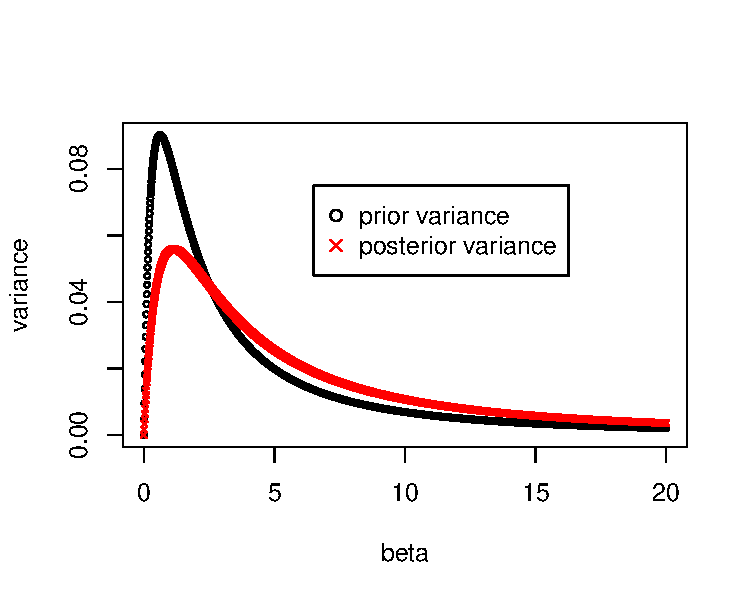
\includegraphics[width=.5\linewidth]{figure/plotbetas-1} 

\end{knitrout}
\end{center}

\end{enumerate}

\item \begin{enumerate}
\item The details of the transformation are shown below. The prior on $log(\theta)$ does not appear to be non-informative. An exponential ``prior'' (I put prior in quotes because it is an improper prior) gives larger values of $log(\theta)$ higher probability. Small and negative values of $log(\theta)$ are given lower probability.
\begin{align*}
p_\theta(\theta)&=1I(\theta)_{(0,\infty)} \\
Y&=log(\theta) \rightarrow e^y=\theta \rightarrow \frac{d\theta}{dy}=e^y \\
f_Y(y) &= p_\theta(e^y)*e^y = 1I(e^y)_{(0,\inf)}e^y \\
f_Y(y) &= e^y I(y)_{(-\infty, \infty)}
\end{align*}

\item To get Jeffrey's non-informative prior density, we find the Fisher Information:
\begin{align*}
-E[\frac{d^2}{d\theta^2}logp(y|\theta)] &= -E[\frac{d^2}{d\theta^2}log(\frac{\theta^ye^{-\theta}}{y!})] \\
&= -E[\frac{d^2}{d\theta^2}ylog\theta-\theta-log(y!)] \\
&= -E[-\frac{y}{\theta^2}] = \frac{1}{\theta} I(\theta)_{(0,\infty)}
\end{align*}
This is the kernel of a $Gam(1/2, 0)$ distribution, but it is an improper prior because it does not have the correct constant to ensure that the density sums to $1$ over the support.

\end{enumerate}

\newpage

\item I am using the previously discussed result that for a binomial pmf with $y$ success in $m$ trials and a $Beta(\alpha, \beta)$ prior, the posterior is $Beta(y+\alpha, m-y+\beta)$. 


\begin{table}[!h]
\begin{tabular}{c|c|c|c}
Prior & Posterior m=6, y=2 & Posterior m=30, y=10 & Posterior m=90, y=30 \\
\hline
Beta(1, 1) & Beta(3, 5) &  Beta(11,21) & Beta(31,61)\\
Beta(0.5, 0.5) & Beta(2.5, 4.5) & Beta(10.5,20.5) & Beta(30.5, 60.5) \\
Beta(2, 2) & Beta(4, 6) & Beta(12, 22) & Beta(32, 62) \\
Beta(0, 0) & Beta(2, 4) & Beta(10, 20) & Beta(30, 60)
\end{tabular}
\end{table}


\begin{knitrout}\footnotesize
\definecolor{shadecolor}{rgb}{0.969, 0.969, 0.969}\color{fgcolor}
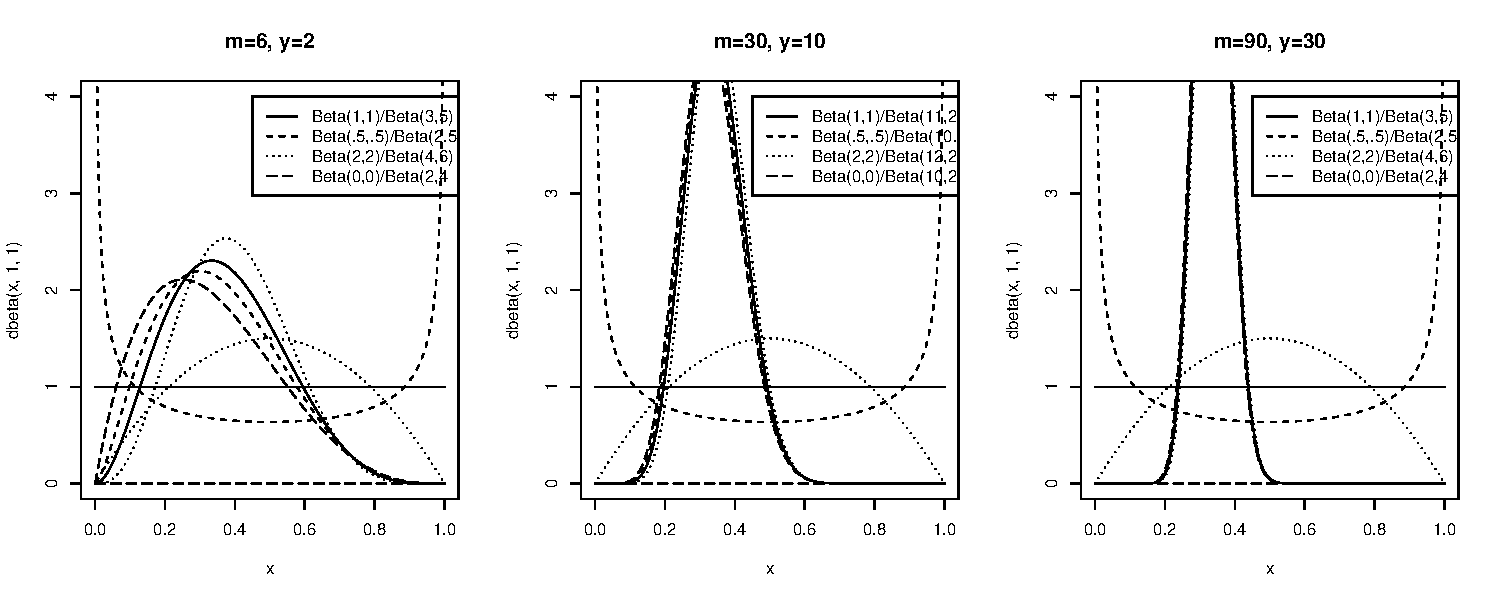
\includegraphics[width=\linewidth]{figure/plotbetaslast-1} 

\end{knitrout}

The plots show the four prior/posterior pairs for each sample size. I think the thing that stands out most from the plots is that the posterior is a lot more sensitive to the prior for smaller $m$ and $y$. As far comparing sensitivity across {\it priors}, it's kind of hard to tell. None of the posterior distributions look too much like the corresponding prior. The $Beta(2,2)$ is closest in shape to the corresponding posterior distribution.



\item  I've always thought that a statement or decision is subjective if someone's personal beliefs are involved. I think there is a gray area, however, when personal beliefs are combined with more objective statements. Consider the example I gave in question $1$ about Serena Williams. If I say that there is a $90\%$ chance that Serena will win the US Open, this reflects both the objective fact that she has won 13 Grand Slam titles, and it reflects my personal belief that she is an incredible tennis player. It seems like there is a similar gray area in choosing prior distributions. The choice of prior may be based on some objective facts, but also incorporates personal beliefs. I think of subjectivity on a spectrum with some statements or decisions incorporating more subjectivity than others. Practically, if I'm trying to decide whether something is more subjective or objective, I think of whether two different reasonable people could arrive at different conclusions and both justify their thought processes.

Steps of Statistical Inference:
\begin{enumerate}
\item Define a research question!! (subjective, way question is defined can be different for different people)
\item Define and think about your explanatory and response variables (objective, all of my 217 students have the same answer for this one and if they don't I mark it wrong)
\item Look at and plot the raw data (subjective. many different reasonable ways to plot data)
\item Decide what to do with missing data, or decide if any observations should not be included (subjective. there could be many different reasonable ideas about what to do with the observation that was taken when the bird had a wet beak)
\item think about potential statistical procedures that could be appropriate (subjective, many different procedures could be justified)
\item check assumptions (subjective, some may have differing ideas about when a violation is severe enough to interfere with the statistical procedures)
\item select a final model, graph, or other to use for inference (subjective, same reason as (e))
\item make a conclusion to address the question of interest (subjective wording. use a p-value cutoff or a strength of evidence statement?)
\item provide estimates for effects of interest (I would call the actual reporting of the estimate objective)
\item describe the scope of inference (subjective - there are general rules about when the design buys inference to the population or causality, but often, even when we don't have a random sample or random assignment we can justify inference to a larger population (or not) based off other knowledge)
\end{enumerate}

\end{enumerate}

\end{doublespacing}

{\bf \Large R Code Appendix}
\begin{knitrout}\footnotesize
\definecolor{shadecolor}{rgb}{0.969, 0.969, 0.969}\color{fgcolor}\begin{kframe}
\begin{alltt}
\hlkwd{require}\hlstd{(ggplot2)}
\hlstd{x} \hlkwb{<-} \hlkwd{seq}\hlstd{(}\hlnum{0}\hlstd{,}\hlnum{1}\hlstd{,} \hlkwc{by}\hlstd{=}\hlnum{0.01}\hlstd{)}
\hlstd{y} \hlkwb{<-} \hlkwd{c}\hlstd{(}\hlkwd{dbeta}\hlstd{(x,}\hlnum{0.5}\hlstd{,}\hlnum{0.5}\hlstd{),} \hlkwd{dbeta}\hlstd{(x,}\hlnum{1}\hlstd{,}\hlnum{1}\hlstd{),} \hlkwd{dbeta}\hlstd{(x,}\hlnum{2}\hlstd{,}\hlnum{2}\hlstd{),} \hlkwd{dbeta}\hlstd{(x,}\hlnum{5}\hlstd{,}\hlnum{5}\hlstd{))}
\hlstd{beta} \hlkwb{<-} \hlkwd{c}\hlstd{(}\hlkwd{rep}\hlstd{(}\hlstr{"(0.5, 0.5)"}\hlstd{,} \hlnum{101}\hlstd{),} \hlkwd{rep}\hlstd{(}\hlstr{"(1, 1)"}\hlstd{,} \hlnum{101}\hlstd{),} \hlkwd{rep}\hlstd{(}\hlstr{"(2, 2)"}\hlstd{,} \hlnum{101}\hlstd{),} \hlkwd{rep}\hlstd{(}\hlstr{"(5, 5)"}\hlstd{,} \hlnum{101}\hlstd{))}
\hlstd{z} \hlkwb{<-} \hlkwd{cbind.data.frame}\hlstd{(x,y, beta)}
\hlkwd{ggplot}\hlstd{(}\hlkwd{aes}\hlstd{(x, y,} \hlkwc{group}\hlstd{=beta),} \hlkwc{data}\hlstd{=z)} \hlopt{+}
  \hlkwd{geom_line}\hlstd{(}\hlkwd{aes}\hlstd{(}\hlkwc{color}\hlstd{=beta,} \hlkwc{size}\hlstd{=beta))}\hlopt{+}
  \hlkwd{xlab}\hlstd{(}\hlstr{""}\hlstd{)}\hlopt{+}
  \hlkwd{ylab}\hlstd{(}\hlstr{""}\hlstd{)}\hlopt{+}
  \hlkwd{ggtitle}\hlstd{(}\hlstr{"Beta"}\hlstd{)}
\end{alltt}
\end{kframe}
\end{knitrout}

\begin{knitrout}\footnotesize
\definecolor{shadecolor}{rgb}{0.969, 0.969, 0.969}\color{fgcolor}\begin{kframe}
\begin{alltt}
\hlkwd{require}\hlstd{(ggplot2)}
\hlstd{x} \hlkwb{<-} \hlkwd{seq}\hlstd{(}\hlnum{0}\hlstd{,}\hlnum{5}\hlstd{,} \hlkwc{by}\hlstd{=}\hlnum{0.05}\hlstd{)}
\hlstd{y} \hlkwb{<-} \hlkwd{c}\hlstd{(}\hlkwd{dgamma}\hlstd{(x,}\hlnum{0.5}\hlstd{,}\hlnum{0.5}\hlstd{),} \hlkwd{dgamma}\hlstd{(x,}\hlnum{1}\hlstd{,}\hlnum{1}\hlstd{),} \hlkwd{dgamma}\hlstd{(x,}\hlnum{2}\hlstd{,}\hlnum{2}\hlstd{),} \hlkwd{dgamma}\hlstd{(x,}\hlnum{5}\hlstd{,}\hlnum{5}\hlstd{))}
\hlstd{gamma} \hlkwb{<-} \hlkwd{c}\hlstd{(}\hlkwd{rep}\hlstd{(}\hlstr{"(2, 2)"}\hlstd{,} \hlnum{101}\hlstd{),} \hlkwd{rep}\hlstd{(}\hlstr{"(1, 1)"}\hlstd{,} \hlnum{101}\hlstd{),} \hlkwd{rep}\hlstd{(}\hlstr{"(1/2, 1/2)"}\hlstd{,} \hlnum{101}\hlstd{),} \hlkwd{rep}\hlstd{(}\hlstr{"(1/5, 1/5)"}\hlstd{,} \hlnum{101}\hlstd{))}
\hlstd{z} \hlkwb{<-} \hlkwd{cbind.data.frame}\hlstd{(x,y, gamma)}
\hlkwd{ggplot}\hlstd{(}\hlkwd{aes}\hlstd{(x, y,} \hlkwc{group}\hlstd{=gamma),} \hlkwc{data}\hlstd{=z)} \hlopt{+}
  \hlkwd{geom_line}\hlstd{(}\hlkwd{aes}\hlstd{(}\hlkwc{color}\hlstd{=gamma,} \hlkwc{size}\hlstd{=gamma))}\hlopt{+}
  \hlkwd{xlab}\hlstd{(}\hlstr{""}\hlstd{)}\hlopt{+}
  \hlkwd{ylab}\hlstd{(}\hlstr{""}\hlstd{)}\hlopt{+}
  \hlkwd{ggtitle}\hlstd{(}\hlstr{"Gamma"}\hlstd{)}
\end{alltt}
\end{kframe}
\end{knitrout}

\begin{knitrout}\footnotesize
\definecolor{shadecolor}{rgb}{0.969, 0.969, 0.969}\color{fgcolor}\begin{kframe}
\begin{alltt}
\hlkwd{require}\hlstd{(ggplot2)}
\hlstd{x} \hlkwb{<-} \hlkwd{seq}\hlstd{(}\hlnum{0}\hlstd{,}\hlnum{0.2}\hlstd{,} \hlkwc{by}\hlstd{=}\hlnum{0.001}\hlstd{)}
\hlstd{y} \hlkwb{<-} \hlkwd{c}\hlstd{(}\hlkwd{dnorm}\hlstd{(x,}\hlnum{0.05}\hlstd{,}\hlnum{0.01}\hlstd{),} \hlkwd{dnorm}\hlstd{(x,} \hlnum{0.10}\hlstd{,} \hlnum{0.01}\hlstd{))}
\hlstd{normal} \hlkwb{<-} \hlkwd{c}\hlstd{(}\hlkwd{rep}\hlstd{(}\hlstr{"N(0.05, 0.01)"}\hlstd{,} \hlnum{201}\hlstd{),} \hlkwd{rep}\hlstd{(}\hlstr{"N(0.10, 0.01)"}\hlstd{,} \hlnum{201}\hlstd{))}
\hlstd{z} \hlkwb{<-} \hlkwd{cbind.data.frame}\hlstd{(x,y, normal)}
\hlkwd{ggplot}\hlstd{(}\hlkwd{aes}\hlstd{(x, y,} \hlkwc{group}\hlstd{=normal),} \hlkwc{data}\hlstd{=z)} \hlopt{+}
  \hlkwd{geom_line}\hlstd{(}\hlkwd{aes}\hlstd{(}\hlkwc{color}\hlstd{=normal,} \hlkwc{size}\hlstd{=normal))}\hlopt{+}
  \hlkwd{xlab}\hlstd{(}\hlstr{"Infection Rate"}\hlstd{)}\hlopt{+}
  \hlkwd{ylab}\hlstd{(}\hlstr{""}\hlstd{)}\hlopt{+}
  \hlkwd{ggtitle}\hlstd{(}\hlstr{"Posterior Distribution of Infection Rates"}\hlstd{)}
\end{alltt}
\end{kframe}
\end{knitrout}

\begin{knitrout}\footnotesize
\definecolor{shadecolor}{rgb}{0.969, 0.969, 0.969}\color{fgcolor}\begin{kframe}
\begin{alltt}
\hlkwd{require}\hlstd{(ggplot2)}
\hlstd{x} \hlkwb{<-} \hlkwd{seq}\hlstd{(}\hlnum{0.48}\hlstd{,}\hlnum{0.50}\hlstd{,} \hlkwc{by}\hlstd{=}\hlnum{0.0001}\hlstd{)}
\hlstd{y} \hlkwb{<-} \hlkwd{dbeta}\hlstd{(x,} \hlnum{241947}\hlstd{,} \hlnum{251529}\hlstd{)}
\hlstd{z} \hlkwb{<-} \hlkwd{cbind.data.frame}\hlstd{(x,y)}
\hlkwd{ggplot}\hlstd{(}\hlkwd{aes}\hlstd{(x, y),} \hlkwc{data}\hlstd{=z)} \hlopt{+}
  \hlkwd{geom_line}\hlstd{()}\hlopt{+}
  \hlkwd{xlab}\hlstd{(}\hlstr{"theta"}\hlstd{)}\hlopt{+}
  \hlkwd{ylab}\hlstd{(}\hlstr{""}\hlstd{)}
\hlcom{#pbeta(0.5, 241947, 251529)}
\end{alltt}
\end{kframe}
\end{knitrout}

\begin{knitrout}\footnotesize
\definecolor{shadecolor}{rgb}{0.969, 0.969, 0.969}\color{fgcolor}\begin{kframe}
\begin{alltt}
\hlkwd{require}\hlstd{(ggplot2)}
\hlkwd{set.seed}\hlstd{(}\hlnum{99}\hlstd{)}
\hlstd{x} \hlkwb{<-} \hlkwd{rpois}\hlstd{(}\hlnum{20}\hlstd{,} \hlnum{5}\hlstd{)}

\hlcom{#write a likelihood function}
\hlstd{poislikelihood} \hlkwb{<-} \hlkwa{function}\hlstd{(}\hlkwc{lambda}\hlstd{) \{}\hlkwd{exp}\hlstd{(}\hlopt{-}\hlnum{20}\hlopt{*}\hlstd{lambda)}\hlopt{*}\hlstd{lambda}\hlopt{^}\hlkwd{sum}\hlstd{(x)}\hlopt{/}\hlkwd{prod}\hlstd{(}\hlkwd{factorial}\hlstd{(x))\}}
\hlstd{lambda} \hlkwb{<-} \hlkwd{seq}\hlstd{(}\hlnum{1}\hlstd{,}\hlnum{10}\hlstd{,} \hlkwc{by}\hlstd{=}\hlnum{0.01}\hlstd{)}

\hlcom{#find mle and endpoints of confidence interval}
\hlkwd{require}\hlstd{(stats)}
\hlstd{mle} \hlkwb{<-} \hlkwd{optimize}\hlstd{(poislikelihood,} \hlkwd{c}\hlstd{(}\hlnum{2.5}\hlstd{,} \hlnum{7.5}\hlstd{),} \hlkwc{maximum}\hlstd{=}\hlnum{TRUE}\hlstd{)}\hlopt{$}\hlstd{maximum}
\hlstd{values} \hlkwb{<-} \hlkwd{optimize}\hlstd{(poislikelihood,} \hlkwd{c}\hlstd{(}\hlnum{2.5}\hlstd{,} \hlnum{7.5}\hlstd{),} \hlkwc{maximum}\hlstd{=}\hlnum{TRUE}\hlstd{)}\hlopt{$}\hlstd{objective}\hlopt{*}\hlnum{0.05}
\hlkwd{require}\hlstd{(mosaic)}
\hlstd{ci.l} \hlkwb{<-} \hlkwd{findZeros}\hlstd{(}\hlkwd{poislikelihood}\hlstd{(lambda)}\hlopt{-}\hlstd{values} \hlopt{~} \hlstd{lambda,} \hlkwc{near}\hlstd{=}\hlnum{0}\hlstd{)[}\hlnum{1}\hlstd{,]}
\hlstd{ci.u} \hlkwb{<-} \hlkwd{findZeros}\hlstd{(}\hlkwd{poislikelihood}\hlstd{(lambda)}\hlopt{-}\hlstd{values} \hlopt{~} \hlstd{lambda,} \hlkwc{near}\hlstd{=}\hlnum{0}\hlstd{)[}\hlnum{2}\hlstd{,]}

\hlcom{#organize into a dataframe and plot}
\hlstd{parta} \hlkwb{<-} \hlkwd{cbind.data.frame}\hlstd{(lambda,} \hlkwc{likelihood}\hlstd{=}\hlkwd{poislikelihood}\hlstd{(lambda))}
\hlkwd{ggplot}\hlstd{(}\hlkwd{aes}\hlstd{(lambda, likelihood),} \hlkwc{data}\hlstd{=parta)}\hlopt{+}
  \hlkwd{geom_line}\hlstd{()}\hlopt{+}
  \hlkwd{geom_vline}\hlstd{(}\hlkwc{xintercept}\hlstd{=mle,} \hlkwc{color}\hlstd{=}\hlstr{"red"}\hlstd{,} \hlkwc{linetype}\hlstd{=}\hlstr{"dashed"}\hlstd{)}\hlopt{+}
  \hlkwd{geom_vline}\hlstd{(}\hlkwc{xintercept}\hlstd{=}\hlnum{5}\hlstd{,} \hlkwc{color}\hlstd{=}\hlstr{"blue"}\hlstd{,} \hlkwc{linetype}\hlstd{=}\hlstr{"dotdash"}\hlstd{)}\hlopt{+}
  \hlkwd{geom_vline}\hlstd{(}\hlkwc{xintercept}\hlstd{=ci.l,} \hlkwc{color}\hlstd{=}\hlstr{"purple"}\hlstd{)}\hlopt{+}
  \hlkwd{geom_vline}\hlstd{(}\hlkwc{xintercept}\hlstd{=ci.u,} \hlkwc{color}\hlstd{=}\hlstr{"purple"}\hlstd{)}
\end{alltt}
\end{kframe}
\end{knitrout}

\begin{knitrout}\footnotesize
\definecolor{shadecolor}{rgb}{0.969, 0.969, 0.969}\color{fgcolor}\begin{kframe}
\begin{alltt}
\hlkwd{require}\hlstd{(ggplot2)}
\hlkwd{set.seed}\hlstd{(}\hlnum{99}\hlstd{)}
\hlstd{x} \hlkwb{<-} \hlkwd{rpois}\hlstd{(}\hlnum{100}\hlstd{,} \hlnum{5}\hlstd{)}

\hlcom{#write a likelihood function}
\hlstd{poisloglikelihood} \hlkwb{<-} \hlkwa{function}\hlstd{(}\hlkwc{lambda}\hlstd{) \{((}\hlopt{-}\hlnum{100}\hlopt{*}\hlstd{lambda)}\hlopt{+}\hlkwd{sum}\hlstd{(x)}\hlopt{*}\hlkwd{log}\hlstd{(lambda))}\hlopt{-}\hlstd{(}\hlkwd{sum}\hlstd{(}\hlkwd{log}\hlstd{(}\hlkwd{factorial}\hlstd{(x))))\}}
\hlstd{poislikelihood100} \hlkwb{<-} \hlkwa{function}\hlstd{(}\hlkwc{lambda}\hlstd{) \{}\hlkwd{exp}\hlstd{(}\hlkwd{poisloglikelihood}\hlstd{(lambda))\}}
\hlstd{lambda} \hlkwb{<-} \hlkwd{seq}\hlstd{(}\hlnum{4}\hlstd{,}\hlnum{6}\hlstd{,} \hlkwc{by}\hlstd{=}\hlnum{0.01}\hlstd{)}

\hlcom{#find mle and endpoints of confidence interval}
\hlkwd{require}\hlstd{(stats)}
\hlstd{mle} \hlkwb{<-} \hlkwd{optimize}\hlstd{(poislikelihood100,} \hlkwd{c}\hlstd{(}\hlnum{2.5}\hlstd{,} \hlnum{7.5}\hlstd{),} \hlkwc{maximum}\hlstd{=}\hlnum{TRUE}\hlstd{)}\hlopt{$}\hlstd{maximum}
\hlstd{values} \hlkwb{<-} \hlkwd{optimize}\hlstd{(poislikelihood100,} \hlkwd{c}\hlstd{(}\hlnum{2.5}\hlstd{,} \hlnum{7.5}\hlstd{),} \hlkwc{maximum}\hlstd{=}\hlnum{TRUE}\hlstd{)}\hlopt{$}\hlstd{objective}\hlopt{*}\hlnum{0.05}
\hlkwd{require}\hlstd{(mosaic)}
\hlstd{ci.l} \hlkwb{<-} \hlkwd{findZeros}\hlstd{(}\hlkwd{poislikelihood100}\hlstd{(lambda)}\hlopt{-}\hlstd{values} \hlopt{~} \hlstd{lambda,} \hlkwc{near}\hlstd{=}\hlnum{0}\hlstd{)[}\hlnum{1}\hlstd{,]}
\hlstd{ci.u} \hlkwb{<-} \hlkwd{findZeros}\hlstd{(}\hlkwd{poislikelihood100}\hlstd{(lambda)}\hlopt{-}\hlstd{values} \hlopt{~} \hlstd{lambda,} \hlkwc{near}\hlstd{=}\hlnum{0}\hlstd{)[}\hlnum{2}\hlstd{,]}

\hlcom{#organize into a dataframe and plot}
\hlstd{partb} \hlkwb{<-} \hlkwd{cbind.data.frame}\hlstd{(lambda,} \hlkwc{likelihood}\hlstd{=}\hlkwd{poislikelihood100}\hlstd{(lambda))}
\hlkwd{ggplot}\hlstd{(}\hlkwd{aes}\hlstd{(lambda, likelihood),} \hlkwc{data}\hlstd{=partb)}\hlopt{+}
  \hlkwd{geom_line}\hlstd{()}\hlopt{+}
  \hlkwd{geom_vline}\hlstd{(}\hlkwc{xintercept}\hlstd{=mle,} \hlkwc{color}\hlstd{=}\hlstr{"red"}\hlstd{,} \hlkwc{linetype}\hlstd{=}\hlstr{"dashed"}\hlstd{)}\hlopt{+}
  \hlkwd{geom_vline}\hlstd{(}\hlkwc{xintercept}\hlstd{=}\hlnum{5}\hlstd{,} \hlkwc{color}\hlstd{=}\hlstr{"blue"}\hlstd{,} \hlkwc{linetype}\hlstd{=}\hlstr{"dotdash"}\hlstd{)}\hlopt{+}
  \hlkwd{geom_vline}\hlstd{(}\hlkwc{xintercept}\hlstd{=ci.l,} \hlkwc{color}\hlstd{=}\hlstr{"purple"}\hlstd{)}\hlopt{+}
  \hlkwd{geom_vline}\hlstd{(}\hlkwc{xintercept}\hlstd{=ci.u,} \hlkwc{color}\hlstd{=}\hlstr{"purple"}\hlstd{)}
\end{alltt}
\end{kframe}
\end{knitrout}

\begin{knitrout}\footnotesize
\definecolor{shadecolor}{rgb}{0.969, 0.969, 0.969}\color{fgcolor}\begin{kframe}
\begin{alltt}
\hlkwd{require}\hlstd{(ggplot2)}
\hlkwd{set.seed}\hlstd{(}\hlnum{55}\hlstd{)}
\hlstd{x} \hlkwb{<-} \hlkwd{rnorm}\hlstd{(}\hlnum{15}\hlstd{,} \hlnum{10}\hlstd{,} \hlkwd{sqrt}\hlstd{(}\hlnum{5}\hlstd{))}

\hlcom{#write a likelihood function}
\hlstd{normloglikelihood} \hlkwb{<-} \hlkwa{function}\hlstd{(}\hlkwc{vec}\hlstd{) \{}
  \hlopt{-}\hlnum{15}\hlopt{/}\hlnum{2}\hlopt{*}\hlkwd{log}\hlstd{(}\hlnum{2}\hlopt{*}\hlstd{pi)}\hlopt{-}\hlnum{15}\hlopt{/}\hlnum{2}\hlopt{*}\hlkwd{log}\hlstd{(vec[}\hlnum{2}\hlstd{])}\hlopt{-}\hlnum{1}\hlopt{/}\hlstd{(}\hlnum{2}\hlopt{*}\hlstd{vec[}\hlnum{2}\hlstd{])}\hlopt{*}\hlkwd{sum}\hlstd{((x}\hlopt{-}\hlstd{vec[}\hlnum{1}\hlstd{])}\hlopt{^}\hlnum{2}\hlstd{)}
\hlstd{\}}
\hlstd{normlikelihood} \hlkwb{<-} \hlkwa{function}\hlstd{(}\hlkwc{vec}\hlstd{) \{}\hlkwd{exp}\hlstd{(}\hlkwd{normloglikelihood}\hlstd{(vec))\}}
\hlstd{vec} \hlkwb{<-} \hlkwd{c}\hlstd{(}\hlnum{5}\hlstd{,}\hlnum{10}\hlstd{)}

\hlcom{#find mle and endpoints of confidence interval}
\hlkwd{require}\hlstd{(stats)}
\hlstd{mles} \hlkwb{<-} \hlkwd{optim}\hlstd{(}\hlkwd{c}\hlstd{(}\hlnum{5}\hlstd{,}\hlnum{3}\hlstd{), normloglikelihood,} \hlkwc{control} \hlstd{=} \hlkwd{list}\hlstd{(}\hlkwc{fnscale} \hlstd{=} \hlopt{-}\hlnum{1}\hlstd{))}\hlopt{$}\hlstd{par}

\hlstd{values} \hlkwb{<-} \hlkwd{exp}\hlstd{(}\hlkwd{optim}\hlstd{(}\hlkwd{c}\hlstd{(}\hlnum{5}\hlstd{,}\hlnum{3}\hlstd{), normloglikelihood,} \hlkwc{control} \hlstd{=} \hlkwd{list}\hlstd{(}\hlkwc{fnscale} \hlstd{=} \hlopt{-}\hlnum{1}\hlstd{))}\hlopt{$}\hlstd{value)}\hlopt{*}\hlnum{0.05}

\hlstd{normloglikelihood2} \hlkwb{<-} \hlkwa{function}\hlstd{(}\hlkwc{mu}\hlstd{,} \hlkwc{sigmasq}\hlstd{) \{}
  \hlopt{-}\hlnum{15}\hlopt{/}\hlnum{2}\hlopt{*}\hlkwd{log}\hlstd{(}\hlnum{2}\hlopt{*}\hlstd{pi)}\hlopt{-}\hlnum{15}\hlopt{/}\hlnum{2}\hlopt{*}\hlkwd{log}\hlstd{(sigmasq)}\hlopt{-}\hlnum{1}\hlopt{/}\hlstd{(}\hlnum{2}\hlopt{*}\hlstd{sigmasq)}\hlopt{*}\hlkwd{sum}\hlstd{((x}\hlopt{-}\hlstd{mu)}\hlopt{^}\hlnum{2}\hlstd{)}
\hlstd{\}}
\hlstd{normlikelihood2} \hlkwb{<-} \hlkwa{function}\hlstd{(}\hlkwc{mu}\hlstd{,} \hlkwc{sigmasq}\hlstd{) \{}\hlkwd{exp}\hlstd{(}\hlkwd{normloglikelihood2}\hlstd{(mu, sigmasq))\}}

\hlkwd{require}\hlstd{(mosaic)}
\hlstd{muci.l} \hlkwb{<-} \hlkwd{findZeros}\hlstd{(}\hlkwd{normlikelihood2}\hlstd{(mu, sigmasq)}\hlopt{-}\hlstd{values} \hlopt{~} \hlstd{mu,} \hlkwc{near}\hlstd{=}\hlnum{0}\hlstd{,} \hlkwc{sigmasq}\hlstd{=}\hlnum{3.299682}\hlstd{)[}\hlnum{1}\hlstd{,]}
\hlstd{muci.u} \hlkwb{<-} \hlkwd{findZeros}\hlstd{(}\hlkwd{normlikelihood2}\hlstd{(mu, sigmasq)}\hlopt{-}\hlstd{values} \hlopt{~} \hlstd{mu,} \hlkwc{near}\hlstd{=}\hlnum{0}\hlstd{,} \hlkwc{sigmasq}\hlstd{=}\hlnum{3.299682}\hlstd{)[}\hlnum{2}\hlstd{,]}

\hlstd{sigmasqci.l} \hlkwb{<-} \hlkwd{findZeros}\hlstd{(}\hlkwd{normlikelihood2}\hlstd{(mu, sigmasq)}\hlopt{-}\hlstd{values} \hlopt{~} \hlstd{sigmasq,} \hlkwc{near}\hlstd{=}\hlnum{0}\hlstd{,} \hlkwc{mu}\hlstd{=}\hlnum{9.1744}\hlstd{)[}\hlnum{1}\hlstd{,]}
\hlstd{sigmasqci.u} \hlkwb{<-} \hlkwd{findZeros}\hlstd{(}\hlkwd{normlikelihood2}\hlstd{(mu, sigmasq)}\hlopt{-}\hlstd{values} \hlopt{~} \hlstd{sigmasq,} \hlkwc{near}\hlstd{=}\hlnum{0}\hlstd{,} \hlkwc{mu}\hlstd{=}\hlnum{9.1744}\hlstd{)[}\hlnum{2}\hlstd{,]}


\hlcom{#contour plot}
\hlstd{ndim} \hlkwb{<-} \hlnum{50}
\hlstd{mu.vals} \hlkwb{<-} \hlstd{mles[}\hlnum{1}\hlstd{]} \hlopt{+} \hlkwd{seq}\hlstd{(}\hlopt{-}\hlnum{5}\hlstd{,}\hlnum{5}\hlstd{,} \hlkwc{length}\hlstd{=ndim)}
\hlstd{sig.vals} \hlkwb{<-} \hlkwd{seq}\hlstd{(}\hlnum{0}\hlstd{, (mles[}\hlnum{2}\hlstd{]} \hlopt{+} \hlnum{12}\hlstd{),} \hlkwc{length}\hlstd{=ndim)}
\hlstd{grid.vals} \hlkwb{<-} \hlkwd{expand.grid}\hlstd{(mu.vals,sig.vals)}
\hlstd{loglik.surf} \hlkwb{<-} \hlkwd{matrix}\hlstd{(}\hlkwd{apply}\hlstd{(grid.vals,}\hlnum{1}\hlstd{,normlikelihood),} \hlkwc{nrow}\hlstd{=ndim,} \hlkwc{ncol}\hlstd{=ndim)}

\hlkwd{contour}\hlstd{(mu.vals, sig.vals, loglik.surf,} \hlkwc{nlevels} \hlstd{=} \hlnum{200}\hlstd{,} \hlkwc{xlab} \hlstd{=} \hlkwd{expression}\hlstd{(mu),}
        \hlkwc{ylab} \hlstd{=} \hlkwd{expression}\hlstd{(sigma),} \hlkwc{main}\hlstd{=}\hlstr{"Likelihood Surface n=15"}\hlstd{,} \hlkwc{xlim}\hlstd{=}\hlkwd{c}\hlstd{(}\hlnum{7.2}\hlstd{,}\hlnum{12}\hlstd{),}
        \hlkwc{ylim}\hlstd{=}\hlkwd{c}\hlstd{(}\hlnum{1}\hlstd{,}\hlnum{13}\hlstd{))}
  \hlkwd{points}\hlstd{(mles[}\hlnum{1}\hlstd{], mles[}\hlnum{2}\hlstd{],} \hlkwc{pch}\hlstd{=}\hlnum{17}\hlstd{,} \hlkwc{col}\hlstd{=}\hlstr{"red"}\hlstd{,} \hlkwc{cex}\hlstd{=}\hlnum{2}\hlstd{)}
  \hlkwd{points}\hlstd{(}\hlnum{10}\hlstd{,} \hlnum{3}\hlstd{,} \hlkwc{pch}\hlstd{=}\hlnum{15}\hlstd{,} \hlkwc{col}\hlstd{=}\hlstr{"blue"}\hlstd{,} \hlkwc{cex}\hlstd{=}\hlnum{2}\hlstd{)}
  \hlkwd{points}\hlstd{(muci.l, sigmasqci.l,} \hlkwc{pch}\hlstd{=}\hlnum{16}\hlstd{,} \hlkwc{col}\hlstd{=}\hlstr{"green"}\hlstd{,} \hlkwc{cex}\hlstd{=}\hlnum{2}\hlstd{)}
  \hlkwd{points}\hlstd{(muci.l, sigmasqci.u,} \hlkwc{pch}\hlstd{=}\hlnum{16}\hlstd{,} \hlkwc{col}\hlstd{=}\hlstr{"green"}\hlstd{,} \hlkwc{cex}\hlstd{=}\hlnum{2}\hlstd{)}
  \hlkwd{points}\hlstd{(muci.u, sigmasqci.l,} \hlkwc{pch}\hlstd{=}\hlnum{16}\hlstd{,} \hlkwc{col}\hlstd{=}\hlstr{"green"}\hlstd{,} \hlkwc{cex}\hlstd{=}\hlnum{2}\hlstd{)}
  \hlkwd{points}\hlstd{(muci.u, sigmasqci.u,} \hlkwc{pch}\hlstd{=}\hlnum{16}\hlstd{,} \hlkwc{col}\hlstd{=}\hlstr{"green"}\hlstd{,} \hlkwc{cex}\hlstd{=}\hlnum{2}\hlstd{)}
  \hlkwd{legend}\hlstd{(}\hlnum{11}\hlstd{,}\hlnum{12}\hlstd{,} \hlkwd{c}\hlstd{(}\hlstr{"CI endpoints"}\hlstd{,} \hlstr{"mle"}\hlstd{,} \hlstr{"truth"}\hlstd{),} \hlkwc{pch}\hlstd{=}\hlkwd{c}\hlstd{(}\hlnum{16}\hlstd{,} \hlnum{17}\hlstd{,} \hlnum{15}\hlstd{))}
\end{alltt}
\end{kframe}
\end{knitrout}

\begin{knitrout}\footnotesize
\definecolor{shadecolor}{rgb}{0.969, 0.969, 0.969}\color{fgcolor}\begin{kframe}
\begin{alltt}
\hlkwd{require}\hlstd{(ggplot2)}
\hlkwd{set.seed}\hlstd{(}\hlnum{55}\hlstd{)}
\hlstd{x} \hlkwb{<-} \hlkwd{rnorm}\hlstd{(}\hlnum{5}\hlstd{,} \hlnum{10}\hlstd{,} \hlkwd{sqrt}\hlstd{(}\hlnum{5}\hlstd{))}

\hlcom{#write a likelihood function}
\hlstd{normloglikelihood} \hlkwb{<-} \hlkwa{function}\hlstd{(}\hlkwc{vec}\hlstd{) \{}
  \hlopt{-}\hlnum{15}\hlopt{/}\hlnum{2}\hlopt{*}\hlkwd{log}\hlstd{(}\hlnum{2}\hlopt{*}\hlstd{pi)}\hlopt{-}\hlnum{15}\hlopt{/}\hlnum{2}\hlopt{*}\hlkwd{log}\hlstd{(vec[}\hlnum{2}\hlstd{])}\hlopt{-}\hlnum{1}\hlopt{/}\hlstd{(}\hlnum{2}\hlopt{*}\hlstd{vec[}\hlnum{2}\hlstd{])}\hlopt{*}\hlkwd{sum}\hlstd{((x}\hlopt{-}\hlstd{vec[}\hlnum{1}\hlstd{])}\hlopt{^}\hlnum{2}\hlstd{)}
\hlstd{\}}
\hlstd{normlikelihood} \hlkwb{<-} \hlkwa{function}\hlstd{(}\hlkwc{vec}\hlstd{) \{}\hlkwd{exp}\hlstd{(}\hlkwd{normloglikelihood}\hlstd{(vec))\}}
\hlstd{vec} \hlkwb{<-} \hlkwd{c}\hlstd{(}\hlnum{5}\hlstd{,}\hlnum{10}\hlstd{)}

\hlcom{#find mle and endpoints of confidence interval}
\hlkwd{require}\hlstd{(stats)}
\hlstd{mles} \hlkwb{<-} \hlkwd{optim}\hlstd{(}\hlkwd{c}\hlstd{(}\hlnum{5}\hlstd{,}\hlnum{3}\hlstd{), normloglikelihood,} \hlkwc{control} \hlstd{=} \hlkwd{list}\hlstd{(}\hlkwc{fnscale} \hlstd{=} \hlopt{-}\hlnum{1}\hlstd{))}\hlopt{$}\hlstd{par}

\hlstd{values} \hlkwb{<-} \hlkwd{exp}\hlstd{(}\hlkwd{optim}\hlstd{(}\hlkwd{c}\hlstd{(}\hlnum{5}\hlstd{,}\hlnum{3}\hlstd{), normloglikelihood,} \hlkwc{control} \hlstd{=} \hlkwd{list}\hlstd{(}\hlkwc{fnscale} \hlstd{=} \hlopt{-}\hlnum{1}\hlstd{))}\hlopt{$}\hlstd{value)}\hlopt{*}\hlnum{0.05}

\hlstd{normloglikelihood2} \hlkwb{<-} \hlkwa{function}\hlstd{(}\hlkwc{mu}\hlstd{,} \hlkwc{sigmasq}\hlstd{) \{}
  \hlopt{-}\hlnum{15}\hlopt{/}\hlnum{2}\hlopt{*}\hlkwd{log}\hlstd{(}\hlnum{2}\hlopt{*}\hlstd{pi)}\hlopt{-}\hlnum{15}\hlopt{/}\hlnum{2}\hlopt{*}\hlkwd{log}\hlstd{(sigmasq)}\hlopt{-}\hlnum{1}\hlopt{/}\hlstd{(}\hlnum{2}\hlopt{*}\hlstd{sigmasq)}\hlopt{*}\hlkwd{sum}\hlstd{((x}\hlopt{-}\hlstd{mu)}\hlopt{^}\hlnum{2}\hlstd{)}
\hlstd{\}}
\hlstd{normlikelihood2} \hlkwb{<-} \hlkwa{function}\hlstd{(}\hlkwc{mu}\hlstd{,} \hlkwc{sigmasq}\hlstd{) \{}\hlkwd{exp}\hlstd{(}\hlkwd{normloglikelihood2}\hlstd{(mu, sigmasq))\}}


\hlkwd{require}\hlstd{(mosaic)}
\hlstd{muci.l} \hlkwb{<-} \hlkwd{findZeros}\hlstd{(}\hlkwd{normlikelihood2}\hlstd{(mu, sigmasq)}\hlopt{-}\hlstd{values} \hlopt{~} \hlstd{mu,} \hlkwc{near}\hlstd{=}\hlnum{0}\hlstd{,} \hlkwc{sigmasq}\hlstd{=}\hlnum{1.054140}\hlstd{)[}\hlnum{1}\hlstd{,]}
\hlstd{muci.u} \hlkwb{<-} \hlkwd{findZeros}\hlstd{(}\hlkwd{normlikelihood2}\hlstd{(mu, sigmasq)}\hlopt{-}\hlstd{values} \hlopt{~} \hlstd{mu,} \hlkwc{near}\hlstd{=}\hlnum{0}\hlstd{,} \hlkwc{sigmasq}\hlstd{=}\hlnum{1.054140}\hlstd{)[}\hlnum{2}\hlstd{,]}

\hlstd{sigmasqci.l} \hlkwb{<-} \hlkwd{findZeros}\hlstd{(}\hlkwd{normlikelihood2}\hlstd{(mu, sigmasq)}\hlopt{-}\hlstd{values} \hlopt{~} \hlstd{sigmasq,} \hlkwc{near}\hlstd{=}\hlnum{0}\hlstd{,} \hlkwc{mu}\hlstd{=}\hlnum{8.811188}\hlstd{)[}\hlnum{1}\hlstd{,]}
\hlstd{sigmasqci.u} \hlkwb{<-} \hlkwd{findZeros}\hlstd{(}\hlkwd{normlikelihood2}\hlstd{(mu, sigmasq)}\hlopt{-}\hlstd{values} \hlopt{~} \hlstd{sigmasq,} \hlkwc{near}\hlstd{=}\hlnum{0}\hlstd{,} \hlkwc{mu}\hlstd{=}\hlnum{8.811188}\hlstd{)[}\hlnum{2}\hlstd{,]}


\hlcom{#contour plot}
\hlstd{ndim} \hlkwb{<-} \hlnum{50}
\hlstd{mu.vals} \hlkwb{<-} \hlstd{mles[}\hlnum{1}\hlstd{]} \hlopt{+} \hlkwd{seq}\hlstd{(}\hlopt{-}\hlnum{5}\hlstd{,}\hlnum{5}\hlstd{,} \hlkwc{length}\hlstd{=ndim)}
\hlstd{sig.vals} \hlkwb{<-} \hlkwd{seq}\hlstd{(}\hlnum{0}\hlstd{, (mles[}\hlnum{2}\hlstd{]} \hlopt{+} \hlnum{12}\hlstd{),} \hlkwc{length}\hlstd{=ndim)}
\hlstd{grid.vals} \hlkwb{<-} \hlkwd{expand.grid}\hlstd{(mu.vals,sig.vals)}
\hlstd{loglik.surf} \hlkwb{<-} \hlkwd{matrix}\hlstd{(}\hlkwd{apply}\hlstd{(grid.vals,}\hlnum{1}\hlstd{,normlikelihood),} \hlkwc{nrow}\hlstd{=ndim,} \hlkwc{ncol}\hlstd{=ndim)}

\hlkwd{contour}\hlstd{(mu.vals, sig.vals, loglik.surf,} \hlkwc{nlevels} \hlstd{=} \hlnum{200}\hlstd{,} \hlkwc{xlab} \hlstd{=} \hlkwd{expression}\hlstd{(mu),}
        \hlkwc{ylab} \hlstd{=} \hlkwd{expression}\hlstd{(sigma),} \hlkwc{main}\hlstd{=}\hlstr{"Likelihood Surface n=5"}\hlstd{,} \hlkwc{xlim}\hlstd{=}\hlkwd{c}\hlstd{(}\hlnum{7.2}\hlstd{,}\hlnum{11}\hlstd{),}
        \hlkwc{ylim}\hlstd{=}\hlkwd{c}\hlstd{(}\hlnum{0}\hlstd{,}\hlnum{6}\hlstd{))}
  \hlkwd{points}\hlstd{(mles[}\hlnum{1}\hlstd{], mles[}\hlnum{2}\hlstd{],} \hlkwc{pch}\hlstd{=}\hlnum{17}\hlstd{,} \hlkwc{col}\hlstd{=}\hlstr{"red"}\hlstd{,} \hlkwc{cex}\hlstd{=}\hlnum{2}\hlstd{)}
  \hlkwd{points}\hlstd{(}\hlnum{10}\hlstd{,} \hlnum{3}\hlstd{,} \hlkwc{pch}\hlstd{=}\hlnum{15}\hlstd{,} \hlkwc{col}\hlstd{=}\hlstr{"blue"}\hlstd{,} \hlkwc{cex}\hlstd{=}\hlnum{2}\hlstd{)}
  \hlkwd{points}\hlstd{(muci.l, sigmasqci.l,} \hlkwc{pch}\hlstd{=}\hlnum{16}\hlstd{,} \hlkwc{col}\hlstd{=}\hlstr{"green"}\hlstd{,} \hlkwc{cex}\hlstd{=}\hlnum{2}\hlstd{)}
  \hlkwd{points}\hlstd{(muci.l, sigmasqci.u,} \hlkwc{pch}\hlstd{=}\hlnum{16}\hlstd{,} \hlkwc{col}\hlstd{=}\hlstr{"green"}\hlstd{,} \hlkwc{cex}\hlstd{=}\hlnum{2}\hlstd{)}
  \hlkwd{points}\hlstd{(muci.u, sigmasqci.l,} \hlkwc{pch}\hlstd{=}\hlnum{16}\hlstd{,} \hlkwc{col}\hlstd{=}\hlstr{"green"}\hlstd{,} \hlkwc{cex}\hlstd{=}\hlnum{2}\hlstd{)}
  \hlkwd{points}\hlstd{(muci.u, sigmasqci.u,} \hlkwc{pch}\hlstd{=}\hlnum{16}\hlstd{,} \hlkwc{col}\hlstd{=}\hlstr{"green"}\hlstd{,} \hlkwc{cex}\hlstd{=}\hlnum{2}\hlstd{)}
  \hlkwd{legend}\hlstd{(}\hlnum{10}\hlstd{,}\hlnum{6}\hlstd{,} \hlkwd{c}\hlstd{(}\hlstr{"CI endpoints"}\hlstd{,} \hlstr{"mle"}\hlstd{,} \hlstr{"truth"}\hlstd{),} \hlkwc{pch}\hlstd{=}\hlkwd{c}\hlstd{(}\hlnum{16}\hlstd{,} \hlnum{17}\hlstd{,} \hlnum{15}\hlstd{))}
\end{alltt}
\end{kframe}
\end{knitrout}

\begin{knitrout}\footnotesize
\definecolor{shadecolor}{rgb}{0.969, 0.969, 0.969}\color{fgcolor}\begin{kframe}
\begin{alltt}
\hlkwd{require}\hlstd{(ggplot2)}
\hlkwd{set.seed}\hlstd{(}\hlnum{55}\hlstd{)}
\hlstd{x} \hlkwb{<-} \hlkwd{rbinom}\hlstd{(}\hlnum{1}\hlstd{,} \hlnum{100}\hlstd{,} \hlnum{0.2}\hlstd{)}

\hlcom{#write a likelihood function}
\hlstd{binomlikelihood} \hlkwb{<-} \hlkwa{function}\hlstd{(}\hlkwc{p}\hlstd{) \{}
  \hlkwd{dbinom}\hlstd{(x,} \hlnum{100}\hlstd{, p)}
\hlstd{\}}

\hlcom{#find mle and endpoints of confidence interval}
\hlkwd{require}\hlstd{(stats)}
\hlstd{mle} \hlkwb{<-} \hlkwd{optimize}\hlstd{(binomlikelihood,} \hlkwd{c}\hlstd{(}\hlnum{.1}\hlstd{,} \hlnum{.3}\hlstd{),} \hlkwc{maximum}\hlstd{=}\hlnum{TRUE}\hlstd{)}\hlopt{$}\hlstd{maximum}

\hlstd{values} \hlkwb{<-} \hlkwd{optimize}\hlstd{(binomlikelihood,} \hlkwd{c}\hlstd{(}\hlnum{.1}\hlstd{,} \hlnum{.3}\hlstd{),} \hlkwc{maximum}\hlstd{=}\hlnum{TRUE}\hlstd{)}\hlopt{$}\hlstd{objective}\hlopt{*}\hlnum{0.05}

\hlkwd{require}\hlstd{(mosaic)}
\hlstd{pci.l} \hlkwb{<-} \hlkwd{findZeros}\hlstd{(}\hlkwd{binomlikelihood}\hlstd{(p)}\hlopt{-}\hlstd{values} \hlopt{~} \hlstd{p,} \hlkwc{near}\hlstd{=}\hlnum{0}\hlstd{)[}\hlnum{1}\hlstd{,]}
\hlstd{pci.u} \hlkwb{<-} \hlkwd{findZeros}\hlstd{(}\hlkwd{binomlikelihood}\hlstd{(p)}\hlopt{-}\hlstd{values} \hlopt{~} \hlstd{p,} \hlkwc{near}\hlstd{=}\hlnum{0}\hlstd{)[}\hlnum{2}\hlstd{,]}

\hlcom{#organize into a dataframe and plot}
\hlstd{p} \hlkwb{<-} \hlkwd{seq}\hlstd{(}\hlnum{0}\hlstd{,} \hlnum{0.4}\hlstd{,} \hlkwc{by}\hlstd{=}\hlnum{0.001}\hlstd{)}
\hlstd{partb} \hlkwb{<-} \hlkwd{cbind.data.frame}\hlstd{(p,} \hlkwc{likelihood}\hlstd{=}\hlkwd{binomlikelihood}\hlstd{(p))}
\hlkwd{ggplot}\hlstd{(}\hlkwd{aes}\hlstd{(p, likelihood),} \hlkwc{data}\hlstd{=partb)}\hlopt{+}
  \hlkwd{geom_line}\hlstd{()}\hlopt{+}
  \hlkwd{geom_vline}\hlstd{(}\hlkwc{xintercept}\hlstd{=mle,} \hlkwc{color}\hlstd{=}\hlstr{"red"}\hlstd{,} \hlkwc{linetype}\hlstd{=}\hlstr{"dashed"}\hlstd{)}\hlopt{+}
  \hlkwd{geom_vline}\hlstd{(}\hlkwc{xintercept}\hlstd{=}\hlnum{.2}\hlstd{,} \hlkwc{color}\hlstd{=}\hlstr{"blue"}\hlstd{,} \hlkwc{linetype}\hlstd{=}\hlstr{"dotdash"}\hlstd{)}\hlopt{+}
  \hlkwd{geom_vline}\hlstd{(}\hlkwc{xintercept}\hlstd{=pci.l,} \hlkwc{color}\hlstd{=}\hlstr{"purple"}\hlstd{)}\hlopt{+}
  \hlkwd{geom_vline}\hlstd{(}\hlkwc{xintercept}\hlstd{=pci.u,} \hlkwc{color}\hlstd{=}\hlstr{"purple"}\hlstd{)}
\end{alltt}
\end{kframe}
\end{knitrout}

\begin{knitrout}\footnotesize
\definecolor{shadecolor}{rgb}{0.969, 0.969, 0.969}\color{fgcolor}\begin{kframe}
\begin{alltt}
\hlkwd{require}\hlstd{(ggplot2)}
\hlkwd{set.seed}\hlstd{(}\hlnum{55}\hlstd{)}
\hlstd{x} \hlkwb{<-} \hlkwd{rbinom}\hlstd{(}\hlnum{30}\hlstd{,} \hlnum{100}\hlstd{,} \hlnum{0.2}\hlstd{)}

\hlcom{#write a likelihood function}
\hlstd{binomloglikelihood} \hlkwb{<-} \hlkwa{function}\hlstd{(}\hlkwc{p}\hlstd{) \{}
  \hlkwd{sum}\hlstd{(}\hlkwd{log}\hlstd{(}\hlkwd{choose}\hlstd{(}\hlnum{100}\hlstd{,x)))}\hlopt{+}\hlkwd{sum}\hlstd{(x)}\hlopt{*}\hlkwd{log}\hlstd{(p)}\hlopt{+}\hlkwd{sum}\hlstd{(}\hlnum{100}\hlopt{-}\hlstd{x)}\hlopt{*}\hlkwd{log}\hlstd{(}\hlnum{1}\hlopt{-}\hlstd{p)}
\hlstd{\}}
\hlstd{binomlikelihood} \hlkwb{<-} \hlkwa{function}\hlstd{(}\hlkwc{p}\hlstd{)\{}\hlkwd{exp}\hlstd{(}\hlkwd{binomloglikelihood}\hlstd{(p))\}}

\hlcom{#find mle and endpoints of confidence interval}
\hlkwd{require}\hlstd{(stats)}
\hlstd{mle} \hlkwb{<-} \hlkwd{optimize}\hlstd{(binomlikelihood,} \hlkwd{c}\hlstd{(}\hlnum{.1}\hlstd{,} \hlnum{.3}\hlstd{),} \hlkwc{maximum}\hlstd{=}\hlnum{TRUE}\hlstd{)}\hlopt{$}\hlstd{maximum}

\hlstd{values} \hlkwb{<-} \hlkwd{optimize}\hlstd{(binomlikelihood,} \hlkwd{c}\hlstd{(}\hlnum{.1}\hlstd{,} \hlnum{.3}\hlstd{),} \hlkwc{maximum}\hlstd{=}\hlnum{TRUE}\hlstd{)}\hlopt{$}\hlstd{objective}\hlopt{*}\hlnum{0.05}

\hlkwd{require}\hlstd{(mosaic)}
\hlstd{pci.l} \hlkwb{<-} \hlkwd{findZeros}\hlstd{(}\hlkwd{binomlikelihood}\hlstd{(p)}\hlopt{-}\hlstd{values} \hlopt{~} \hlstd{p,} \hlkwc{near}\hlstd{=}\hlnum{0}\hlstd{)[}\hlnum{1}\hlstd{,]}
\hlstd{pci.u} \hlkwb{<-} \hlkwd{findZeros}\hlstd{(}\hlkwd{binomlikelihood}\hlstd{(p)}\hlopt{-}\hlstd{values} \hlopt{~} \hlstd{p,} \hlkwc{near}\hlstd{=}\hlnum{0}\hlstd{)[}\hlnum{2}\hlstd{,]}

\hlcom{#organize into a dataframe and plot}
\hlstd{p} \hlkwb{<-} \hlkwd{seq}\hlstd{(}\hlnum{0.1}\hlstd{,} \hlnum{0.3}\hlstd{,} \hlkwc{by}\hlstd{=}\hlnum{0.001}\hlstd{)}
\hlstd{partb} \hlkwb{<-} \hlkwd{cbind.data.frame}\hlstd{(p,} \hlkwc{likelihood}\hlstd{=}\hlkwd{binomlikelihood}\hlstd{(p))}
\hlkwd{ggplot}\hlstd{(}\hlkwd{aes}\hlstd{(p, likelihood),} \hlkwc{data}\hlstd{=partb)}\hlopt{+}
  \hlkwd{geom_line}\hlstd{()}\hlopt{+}
  \hlkwd{geom_vline}\hlstd{(}\hlkwc{xintercept}\hlstd{=mle,} \hlkwc{color}\hlstd{=}\hlstr{"red"}\hlstd{,} \hlkwc{linetype}\hlstd{=}\hlstr{"dashed"}\hlstd{)}\hlopt{+}
  \hlkwd{geom_vline}\hlstd{(}\hlkwc{xintercept}\hlstd{=}\hlnum{.2}\hlstd{,} \hlkwc{color}\hlstd{=}\hlstr{"blue"}\hlstd{,} \hlkwc{linetype}\hlstd{=}\hlstr{"dotdash"}\hlstd{)}\hlopt{+}
  \hlkwd{geom_vline}\hlstd{(}\hlkwc{xintercept}\hlstd{=pci.l,} \hlkwc{color}\hlstd{=}\hlstr{"purple"}\hlstd{)}\hlopt{+}
  \hlkwd{geom_vline}\hlstd{(}\hlkwc{xintercept}\hlstd{=pci.u,} \hlkwc{color}\hlstd{=}\hlstr{"purple"}\hlstd{)}
\end{alltt}
\end{kframe}
\end{knitrout}

\begin{knitrout}\footnotesize
\definecolor{shadecolor}{rgb}{0.969, 0.969, 0.969}\color{fgcolor}\begin{kframe}
\begin{alltt}
\hlkwd{require}\hlstd{(ggplot2)}
\hlstd{x} \hlkwb{<-} \hlkwd{c}\hlstd{(}\hlopt{-}\hlnum{5}\hlstd{,} \hlnum{8}\hlstd{)}
\hlstd{plot.fun} \hlkwb{<-} \hlkwa{function}\hlstd{(}\hlkwc{x}\hlstd{)\{}
  \hlnum{1}\hlopt{/}\hlstd{(}\hlnum{4}\hlopt{*}\hlkwd{sqrt}\hlstd{(}\hlnum{2}\hlopt{*}\hlstd{pi))}\hlopt{*}\hlstd{(}\hlkwd{exp}\hlstd{(}\hlopt{-}\hlstd{(x}\hlopt{-}\hlnum{1}\hlstd{)}\hlopt{^}\hlnum{2}\hlopt{/}\hlnum{8}\hlstd{)}\hlopt{+}\hlkwd{exp}\hlstd{(}\hlopt{-}\hlstd{(x}\hlopt{-}\hlnum{2}\hlstd{)}\hlopt{^}\hlnum{2}\hlopt{/}\hlnum{8}\hlstd{))}
\hlstd{\}}

\hlstd{y} \hlkwb{<-} \hlkwd{rep}\hlstd{(}\hlnum{0}\hlstd{,}\hlnum{2}\hlstd{)}
\hlkwd{qplot}\hlstd{(x,y)}\hlopt{+}\hlkwd{geom_point}\hlstd{(}\hlkwc{color}\hlstd{=}\hlstr{"white"}\hlstd{)}\hlopt{+}
  \hlkwd{stat_function}\hlstd{(}\hlkwc{fun} \hlstd{= plot.fun,} \hlkwc{colour} \hlstd{=} \hlstr{"red"}\hlstd{)}\hlopt{+}
  \hlkwd{xlab}\hlstd{(}\hlstr{"y"}\hlstd{)}\hlopt{+}
  \hlkwd{ylab}\hlstd{(}\hlstr{"p(y)"}\hlstd{)}
\end{alltt}
\end{kframe}
\end{knitrout}

\begin{knitrout}\footnotesize
\definecolor{shadecolor}{rgb}{0.969, 0.969, 0.969}\color{fgcolor}\begin{kframe}
\begin{alltt}
\hlstd{y} \hlkwb{<-} \hlkwd{c}\hlstd{(}\hlnum{1}\hlopt{/}\hlstd{(}\hlnum{1}\hlopt{+}\hlkwd{exp}\hlstd{(}\hlopt{-}\hlnum{1}\hlopt{/}\hlnum{8}\hlstd{)),} \hlkwd{exp}\hlstd{(}\hlopt{-}\hlnum{1}\hlopt{/}\hlnum{8}\hlstd{)}\hlopt{/}\hlstd{(}\hlnum{1}\hlopt{+}\hlkwd{exp}\hlstd{(}\hlopt{-}\hlnum{1}\hlopt{/}\hlnum{8}\hlstd{)))}
\hlstd{z} \hlkwb{<-} \hlkwd{c}\hlstd{(}\hlnum{1}\hlopt{/}\hlstd{((}\hlnum{1}\hlopt{+}\hlkwd{exp}\hlstd{(}\hlopt{-}\hlnum{1}\hlopt{/}\hlnum{32}\hlstd{))),} \hlkwd{exp}\hlstd{(}\hlopt{-}\hlnum{1}\hlopt{/}\hlnum{32}\hlstd{)}\hlopt{/}\hlstd{((}\hlnum{1}\hlopt{+}\hlkwd{exp}\hlstd{(}\hlopt{-}\hlnum{1}\hlopt{/}\hlnum{32}\hlstd{))))}
\hlstd{f} \hlkwb{<-} \hlkwd{c}\hlstd{(}\hlnum{1}\hlopt{/}\hlstd{((}\hlnum{1}\hlopt{+}\hlkwd{exp}\hlstd{(}\hlopt{-}\hlnum{1}\hlopt{/}\hlnum{2}\hlstd{))),} \hlkwd{exp}\hlstd{(}\hlopt{-}\hlnum{1}\hlopt{/}\hlnum{2}\hlstd{)}\hlopt{/}\hlstd{((}\hlnum{1}\hlopt{+}\hlkwd{exp}\hlstd{(}\hlopt{-}\hlnum{1}\hlopt{/}\hlnum{2}\hlstd{))))}
\hlstd{theta} \hlkwb{<-} \hlkwd{c}\hlstd{(}\hlnum{1}\hlstd{,}\hlnum{2}\hlstd{)}
\hlkwd{plot}\hlstd{(theta, y,} \hlkwc{lwd}\hlstd{=}\hlnum{2}\hlstd{,} \hlkwc{ylim}\hlstd{=}\hlkwd{c}\hlstd{(}\hlnum{0.35}\hlstd{,}\hlnum{0.65}\hlstd{),} \hlkwc{ylab}\hlstd{=}\hlstr{"p(theta|y=1)"}\hlstd{)}
\hlkwd{points}\hlstd{(theta, z,} \hlkwc{pch}\hlstd{=}\hlnum{3}\hlstd{)}
\hlkwd{points}\hlstd{(theta, f,} \hlkwc{pch}\hlstd{=}\hlnum{4}\hlstd{)}
\hlkwd{legend}\hlstd{(}\hlnum{1.6}\hlstd{,}\hlnum{0.46}\hlstd{,} \hlkwd{c}\hlstd{(}\hlstr{"sigma=2"}\hlstd{,} \hlstr{"sigma=4"}\hlstd{,} \hlstr{"sigma=1"}\hlstd{),} \hlkwc{pch}\hlstd{=}\hlkwd{c}\hlstd{(}\hlnum{1}\hlstd{,}\hlnum{3}\hlstd{,}\hlnum{4}\hlstd{))}
\end{alltt}
\end{kframe}
\end{knitrout}

\begin{knitrout}\footnotesize
\definecolor{shadecolor}{rgb}{0.969, 0.969, 0.969}\color{fgcolor}\begin{kframe}
\begin{alltt}
\hlstd{beta} \hlkwb{<-} \hlkwd{seq}\hlstd{(}\hlnum{0}\hlstd{,}\hlnum{20}\hlstd{,} \hlkwc{by}\hlstd{=}\hlnum{0.01}\hlstd{)}
\hlstd{priorvar} \hlkwb{<-} \hlstd{beta}\hlopt{/}\hlstd{((beta}\hlopt{+}\hlnum{1}\hlstd{)}\hlopt{^}\hlnum{2}\hlopt{*}\hlstd{(beta}\hlopt{+}\hlnum{2}\hlstd{))}
\hlstd{postvar} \hlkwb{<-} \hlnum{2}\hlopt{*}\hlstd{beta}\hlopt{/}\hlstd{((beta}\hlopt{+}\hlnum{2}\hlstd{)}\hlopt{^}\hlnum{2}\hlopt{*}\hlstd{(beta}\hlopt{+}\hlnum{3}\hlstd{))}
\hlkwd{plot}\hlstd{(beta, priorvar,} \hlkwc{ylab}\hlstd{=}\hlstr{"variance"}\hlstd{,} \hlkwc{cex}\hlstd{=}\hlnum{0.5}\hlstd{)}
\hlkwd{points}\hlstd{(beta, postvar,} \hlkwc{col}\hlstd{=}\hlstr{"red"}\hlstd{,} \hlkwc{pch}\hlstd{=}\hlnum{4}\hlstd{,} \hlkwc{cex}\hlstd{=}\hlnum{0.5}\hlstd{)}
\hlkwd{legend}\hlstd{(}\hlnum{6.5}\hlstd{,}\hlnum{0.075}\hlstd{,} \hlkwd{c}\hlstd{(}\hlstr{"prior variance"}\hlstd{,} \hlstr{"posterior variance"}\hlstd{),} \hlkwc{pch}\hlstd{=}\hlkwd{c}\hlstd{(}\hlnum{1}\hlstd{,}\hlnum{4}\hlstd{),} \hlkwc{col}\hlstd{=}\hlkwd{c}\hlstd{(}\hlstr{"black"}\hlstd{,} \hlstr{"red"}\hlstd{))}
\end{alltt}
\end{kframe}
\end{knitrout}

\begin{knitrout}\footnotesize
\definecolor{shadecolor}{rgb}{0.969, 0.969, 0.969}\color{fgcolor}\begin{kframe}
\begin{alltt}
\hlkwd{par}\hlstd{(}\hlkwc{mfrow}\hlstd{=}\hlkwd{c}\hlstd{(}\hlnum{1}\hlstd{,}\hlnum{3}\hlstd{))}
\hlstd{x} \hlkwb{<-} \hlkwd{seq}\hlstd{(}\hlnum{0}\hlstd{,}\hlnum{1}\hlstd{,}\hlkwc{by}\hlstd{=}\hlnum{0.001}\hlstd{)}
\hlkwd{plot}\hlstd{(x,} \hlkwd{dbeta}\hlstd{(x,} \hlnum{1}\hlstd{,}\hlnum{1}\hlstd{),} \hlkwc{ylim}\hlstd{=}\hlkwd{c}\hlstd{(}\hlnum{0}\hlstd{,}\hlnum{4}\hlstd{),} \hlkwc{type}\hlstd{=}\hlstr{"l"}\hlstd{,} \hlkwc{main}\hlstd{=}\hlstr{"m=6, y=2"}\hlstd{)}
\hlkwd{lines}\hlstd{(x,} \hlkwd{dbeta}\hlstd{(x,} \hlnum{3}\hlstd{,}\hlnum{5}\hlstd{),} \hlkwc{lty}\hlstd{=}\hlnum{1}\hlstd{)}
\hlkwd{lines}\hlstd{(x,} \hlkwd{dbeta}\hlstd{(x,} \hlnum{.5}\hlstd{,}\hlnum{.5}\hlstd{),} \hlkwc{lty}\hlstd{=}\hlnum{2}\hlstd{)}
\hlkwd{lines}\hlstd{(x,} \hlkwd{dbeta}\hlstd{(x,} \hlnum{2.5}\hlstd{,} \hlnum{4.5}\hlstd{),} \hlkwc{lty}\hlstd{=}\hlnum{2}\hlstd{)}
\hlkwd{lines}\hlstd{(x,} \hlkwd{dbeta}\hlstd{(x,} \hlnum{2}\hlstd{,}\hlnum{2}\hlstd{),} \hlkwc{lty}\hlstd{=}\hlnum{3}\hlstd{)}
\hlkwd{lines}\hlstd{(x,} \hlkwd{dbeta}\hlstd{(x,} \hlnum{4}\hlstd{,} \hlnum{6}\hlstd{),} \hlkwc{lty}\hlstd{=}\hlnum{3}\hlstd{)}
\hlkwd{lines}\hlstd{(x,} \hlkwd{dbeta}\hlstd{(x,} \hlnum{0}\hlstd{,}\hlnum{0}\hlstd{),} \hlkwc{lty}\hlstd{=}\hlnum{5}\hlstd{)}
\hlkwd{lines}\hlstd{(x,} \hlkwd{dbeta}\hlstd{(x,} \hlnum{2}\hlstd{,} \hlnum{4}\hlstd{),} \hlkwc{lty}\hlstd{=}\hlnum{5}\hlstd{)}
\hlkwd{legend}\hlstd{(}\hlnum{0.45}\hlstd{,}\hlnum{4}\hlstd{,} \hlkwd{c}\hlstd{(}\hlstr{"Beta(1,1)/Beta(3,5) Prior/Post"}\hlstd{,} \hlstr{"Beta(.5,.5)/Beta(2.5,4.5)"}\hlstd{,} \hlstr{"Beta(2,2)/Beta(4,6)"}\hlstd{,} \hlstr{"Beta(0,0)/Beta(2,4"}\hlstd{),} \hlkwc{lty}\hlstd{=}\hlkwd{c}\hlstd{(}\hlnum{1}\hlstd{,}\hlnum{2}\hlstd{,}\hlnum{3}\hlstd{,}\hlnum{5}\hlstd{))}

\hlstd{x} \hlkwb{<-} \hlkwd{seq}\hlstd{(}\hlnum{0}\hlstd{,}\hlnum{1}\hlstd{,}\hlkwc{by}\hlstd{=}\hlnum{0.001}\hlstd{)}
\hlkwd{plot}\hlstd{(x,} \hlkwd{dbeta}\hlstd{(x,} \hlnum{1}\hlstd{,}\hlnum{1}\hlstd{),} \hlkwc{ylim}\hlstd{=}\hlkwd{c}\hlstd{(}\hlnum{0}\hlstd{,}\hlnum{4}\hlstd{),} \hlkwc{type}\hlstd{=}\hlstr{"l"}\hlstd{,} \hlkwc{main}\hlstd{=}\hlstr{"m=30, y=10"}\hlstd{)}
\hlkwd{lines}\hlstd{(x,} \hlkwd{dbeta}\hlstd{(x,} \hlnum{11}\hlstd{,}\hlnum{21}\hlstd{),} \hlkwc{lty}\hlstd{=}\hlnum{1}\hlstd{)}
\hlkwd{lines}\hlstd{(x,} \hlkwd{dbeta}\hlstd{(x,} \hlnum{.5}\hlstd{,}\hlnum{.5}\hlstd{),} \hlkwc{lty}\hlstd{=}\hlnum{2}\hlstd{)}
\hlkwd{lines}\hlstd{(x,} \hlkwd{dbeta}\hlstd{(x,} \hlnum{10.5}\hlstd{,} \hlnum{20.5}\hlstd{),} \hlkwc{lty}\hlstd{=}\hlnum{2}\hlstd{)}
\hlkwd{lines}\hlstd{(x,} \hlkwd{dbeta}\hlstd{(x,} \hlnum{2}\hlstd{,}\hlnum{2}\hlstd{),} \hlkwc{lty}\hlstd{=}\hlnum{3}\hlstd{)}
\hlkwd{lines}\hlstd{(x,} \hlkwd{dbeta}\hlstd{(x,} \hlnum{12}\hlstd{,} \hlnum{22}\hlstd{),} \hlkwc{lty}\hlstd{=}\hlnum{3}\hlstd{)}
\hlkwd{lines}\hlstd{(x,} \hlkwd{dbeta}\hlstd{(x,} \hlnum{0}\hlstd{,}\hlnum{0}\hlstd{),} \hlkwc{lty}\hlstd{=}\hlnum{5}\hlstd{)}
\hlkwd{lines}\hlstd{(x,} \hlkwd{dbeta}\hlstd{(x,} \hlnum{10}\hlstd{,} \hlnum{20}\hlstd{),} \hlkwc{lty}\hlstd{=}\hlnum{5}\hlstd{)}
\hlkwd{legend}\hlstd{(}\hlnum{0.45}\hlstd{,}\hlnum{4}\hlstd{,} \hlkwd{c}\hlstd{(}\hlstr{"Beta(1,1)/Beta(11,21) Prior/Post"}\hlstd{,} \hlstr{"Beta(.5,.5)/Beta(10.5,20.5)"}\hlstd{,} \hlstr{"Beta(2,2)/Beta(12,22)"}\hlstd{,} \hlstr{"Beta(0,0)/Beta(10,20"}\hlstd{),} \hlkwc{lty}\hlstd{=}\hlkwd{c}\hlstd{(}\hlnum{1}\hlstd{,}\hlnum{2}\hlstd{,}\hlnum{3}\hlstd{,}\hlnum{5}\hlstd{))}

\hlstd{x} \hlkwb{<-} \hlkwd{seq}\hlstd{(}\hlnum{0}\hlstd{,}\hlnum{1}\hlstd{,}\hlkwc{by}\hlstd{=}\hlnum{0.001}\hlstd{)}
\hlkwd{plot}\hlstd{(x,} \hlkwd{dbeta}\hlstd{(x,} \hlnum{1}\hlstd{,}\hlnum{1}\hlstd{),} \hlkwc{ylim}\hlstd{=}\hlkwd{c}\hlstd{(}\hlnum{0}\hlstd{,}\hlnum{4}\hlstd{),} \hlkwc{type}\hlstd{=}\hlstr{"l"}\hlstd{,} \hlkwc{main}\hlstd{=}\hlstr{"m=90, y=30"}\hlstd{)}
\hlkwd{lines}\hlstd{(x,} \hlkwd{dbeta}\hlstd{(x,} \hlnum{31}\hlstd{,}\hlnum{61}\hlstd{),} \hlkwc{lty}\hlstd{=}\hlnum{1}\hlstd{)}
\hlkwd{lines}\hlstd{(x,} \hlkwd{dbeta}\hlstd{(x,} \hlnum{.5}\hlstd{,}\hlnum{.5}\hlstd{),} \hlkwc{lty}\hlstd{=}\hlnum{2}\hlstd{)}
\hlkwd{lines}\hlstd{(x,} \hlkwd{dbeta}\hlstd{(x,} \hlnum{30.5}\hlstd{,} \hlnum{60.5}\hlstd{),} \hlkwc{lty}\hlstd{=}\hlnum{2}\hlstd{)}
\hlkwd{lines}\hlstd{(x,} \hlkwd{dbeta}\hlstd{(x,} \hlnum{2}\hlstd{,}\hlnum{2}\hlstd{),} \hlkwc{lty}\hlstd{=}\hlnum{3}\hlstd{)}
\hlkwd{lines}\hlstd{(x,} \hlkwd{dbeta}\hlstd{(x,} \hlnum{32}\hlstd{,} \hlnum{62}\hlstd{),} \hlkwc{lty}\hlstd{=}\hlnum{3}\hlstd{)}
\hlkwd{lines}\hlstd{(x,} \hlkwd{dbeta}\hlstd{(x,} \hlnum{0}\hlstd{,}\hlnum{0}\hlstd{),} \hlkwc{lty}\hlstd{=}\hlnum{5}\hlstd{)}
\hlkwd{lines}\hlstd{(x,} \hlkwd{dbeta}\hlstd{(x,} \hlnum{30}\hlstd{,} \hlnum{60}\hlstd{),} \hlkwc{lty}\hlstd{=}\hlnum{5}\hlstd{)}
\hlkwd{legend}\hlstd{(}\hlnum{0.45}\hlstd{,}\hlnum{4}\hlstd{,} \hlkwd{c}\hlstd{(}\hlstr{"Beta(1,1)/Beta(3,5) Prior/Post"}\hlstd{,} \hlstr{"Beta(.5,.5)/Beta(2.5,4.5)"}\hlstd{,} \hlstr{"Beta(2,2)/Beta(4,6)"}\hlstd{,} \hlstr{"Beta(0,0)/Beta(2,4"}\hlstd{),} \hlkwc{lty}\hlstd{=}\hlkwd{c}\hlstd{(}\hlnum{1}\hlstd{,}\hlnum{2}\hlstd{,}\hlnum{3}\hlstd{,}\hlnum{5}\hlstd{))}
\end{alltt}
\end{kframe}
\end{knitrout}
\end{document}
